\documentclass{polytech/polytech}
\newcolumntype{L}[1]{>{\raggedright\arraybackslash}p{#1}}


\typereport{stagedi5}

\reportyear{2017-2018}
\title{Réalisation d'un outil de cartographie sur le progiciel Amplitude}
\student{Romain}{ROUSSEAU}{romain.rousseau@etu.univ-tours.fr}
\academicsupervisor{Yannick}{KERGOSIEN}{yannick.kergosien@univ-tours.fr}
\industrialsupervisor[Responsable Cellule Architecture]{Alexandre}{DURAND}{alexandre.durand@soprabanking.com}

\company[images/logoSopra]{Sopra Banking}{47 rue Christiaan Huygens \\ 37073 Tours Cedex 2 - France}{www.soprabanking.com}

\resume{Le stage de cinquième année d'école d'ingénieur est la dernière expérience avant l'entrée dans la vie active. Mon stage consiste en la mise en place d'un outil de cartographie pour le progiciel bancaire \textit{Amplitude} développé par l'entreprise \textit{Sopra Banking Software}. Le progiciel étant très vaste et complexe à manipuler, la mise en place d'une cartographie permettrait d'améliorer considérablement le quotidien des architectes fonctionnels. L'outil sera une plateforme interne à l'entreprise développée avec des technologies récentes comme \textit{Spring Boot}, \textit{Spring Data} ou encore \textit{Angular}.}

\motcle{stage, outil, cartographie, spring boot, spring data, angular}

\abstract{The internship of the fifth year in engineering school is the last experience before the entrance in the working life. My internship consists in the built of a tool designed for mapping the software package \textit{Amplitude} designed by \textit{Sopra Banking Software}. The software has a very wide range of different fiels, making a map of it would improve the everyday life of the developpers. The tool will be a intern platform for the company developped with new technologies like \textit{Spring Boot}, \textit{Spring Data} or \textit{Angular}.}

\keyword{internship, tool, mapping, spring boot, spring data, angular}


%%%%%%%%%%%%%%%%%%%%%%%%%%%%%%%%%%%%%%%%%%%%%%%%%%%%%%%%%%%%%%%%%%%%%%%%%%%%%%%%%%%%%%%%%%%%%%%%%%%
%%%%%%%%%%%%%%%%%%%%%%%%%%%%%%%%%%%%%%%%%%%%%%%%%%%%%%%%%%%%%%%%%%%%%%%%%%%%%%%%%%%%%%%%%%%%%%%%%%%

\begin{document}

\chapter*{Introduction}


Ce rapport présente mon stage d'assistant ingénieur réalisé dans l'entreprise \textit{Sopra Banking Software} à Tours. Le sujet du stage était la réalisation d'un outil de cartographie pour le progiciel nommé \textit{Amplitude} de l'entreprise. Le stage a débuté le 9 avril 2018 avant de s'achever le 31 août de la même année.

Le stage de cinquième année a pour but d'appliquer les connaissances acquises lors des précédentes années d'étude. Il doit représenter une synthèse de l'ensemble des caractéristiques qu'un ingénieur doit avoir dans un environnement concret. Alors que le stage de troisième année sert à découvrir le monde de l'entreprise et que celui de quatrième année sert à faire le premier pas vers le métier d'ingénieur, le stage de dernière année permet de travailler dans une équipe installée pour mener à bien un projet, dans son intégralité ou tout du moins sa majorité selon les cas. Ce stage est censé donner une autonomie supérieure aux étudiants, qui doivent prendre des décisions et avoir la possibilité de donner leur avis sur les opérations en cours, ce qui en fait ainsi, une expérience nécessaire pour le métier. 

Il se déroule sur une période d'au minimum 18 semaines, ce qui permet de pouvoir réaliser des projets avec une envergure dont les étudiants-ingénieurs n'ont jamais eu l'occasion de faire durant leur cursus. Il s'agit du stage le plus important de la formation car il s'agit du plus complet, du plus formateur et de manière générale, du plus intéressant. Il apporte une expérience non négligeable et représente la dernière marche avant l'arrivée dans la vie active.

Le secteur de l'informatique est très porteur et les offres de stage sont donc très nombreuses et variées. L'opportunité de stage dans l'entreprise \textit{Sopra Banking Software} est venue lors du Forum des Entreprises qui se déroule à Polytech pendant le mois de novembre. J'ai pu y rencontrer de nombreux acteurs du secteur et obtenir des entretiens avec plusieurs d'entre eux, dont notamment deux à Sopra sur le site de Tours. À la suite de ces entretiens, j'ai pu faire mon choix parmi les propositions. J'ai retenu celle de la Cellule Architecture de \textit{Sopra Banking Software} pour plusieurs raisons. Tout d'abord, le domaine de la banque m'a toujours intéressé, j'ai déjà fait mon stage de 4ème année chez Worldline du côté des paiements en ligne et je voulais découvrir un autre aspect du domaine. Ensuite, j'avais envie de faire partie d'un projet que ne soit pas monotone et qui me permette d'acquérir de nouvelles connaissances sur des technologies que je ne maîtrise pas ou très peu. Et c'était le cas avec cette offre qui combinait tous les aspects d'un projet, de l'expression des besoins jusqu'au développement en passant par la modélisation ou encore le chiffrage, le tout en utilisant des technologies récentes, variées et performantes. 

Les chapitres qui vont suivre exposeront les principales phases de mon stage, en commençant d'abord par une présentation de l'entreprise et du projet en lui-même. La suite sera consacrée à mon parcours au sein de l'équipe, avec dans un premier temps, une phase de formation sur les différents éléments de l'entreprise ainsi que sur les technologies qui seront utilisées; puis, à la modélisation de l'outil, avec l'élaboration des diagrammes de Gantt, et le chiffrage du projet; et enfin le développement en lui-même. 

\part{Présentation de l'entreprise et du projet}

Cette partie sera consacrée à la présentation du cadre général de mon stage, c'est-à-dire le groupe \textit{Sopra Steria}, sa filiale \textit{Sopra Banking Software}, le progiciel \textit{Amplitude} et la présentation générale du sujet. 

\chapter{Le groupe \textit{Sopra Steria} et \textit{Sopra Banking Software}}

\section{Histoire des deux groupes: \textit{Sopra} et \textit{Steria}}

\begin{figure}
	
\includegraphics[scale=1]{images/sopralogo}
\end{figure}

\textit{Sopra Steria} est une entreprise de services du numérique qui propose des prestations de conseils, des services technologiques et qui édite des logiciels métiers dans trois principaux domaines: les ressources humaines, l'immobilier et la banque. Définie comme leader européen de la transformation numérique, l'entreprise, de par sa diversité, propose l'un des portefeuilles d'offres les plus complets du marché. L'une des principales motivations du groupe est d'accompagner ses clients dans leur transformation numérique et les aider à faire le meilleur usage de leurs outils. Parmi les actuels clients de l'entreprise, on peut citer des grands noms comme Airbus, La Banque Postale, le Ministère de la Défense, EDF, le Ministère des Finances, la SNCF, Easyjet, et bien d'autres.  

Comme beaucoup de SSII à grandes envergures, \textit{Sopra Steria} est le fruit de nombreuses acquisitions et fusions au fil du temps. Tout d'abord, \textit{Sopra} et \textit{Steria} composaient deux entreprises distinctes. Elles ont toutes les deux été créées à la fin des années 70 (en 1968 pour \textit{Sopra} et en \textit{1968} pour \textit{Steria}). Les deux entreprises se développent dans les années qui suivent. \textit{Sopra} (acronyme pour \textbf{SO}ciété de \textbf{PR}ogrammation et d'\textbf{A}nalyses) investit dans le développement de logiciels, notamment dans le domaine bancaire et les ressources humaines. Le groupe \textit{Sopra} fera son entrée à la bourse de Paris en 1990 après avoir travaillé sur un projet avec Ministère de l'Intérieur. De son côté, \textit{Steria} (acronyme de Société d'étude et de réalisation en informatique et automatisme) réalise de grandes signatures du côté de la sphère publique, en informatisant l'AFP en 1975 ou encore en participant au développement du Minitel en 1981 par exemple. 

Le milieu des années 90 marque le début d'une série d'acquisitions de la part des deux groupes. \textit{Sopra} s'implante au Royaume-Uni, en Espagne, en Italie et en Allemagne en 1999 tandis que \textit{Steria} rentre à la bourse de Paris cette même année. Par la suite, le groupe double de taille en intégrant les activités européennes de \textit{Bull} en 2001 et se renforce dans le conseil en acquérant l'entreprise allemande \textit{Mummert Consulting} en 2005. \textit{Steria} développera considérablement ses parts de marché dans le secteur public au Royaume-Uni en acquérant la société \textit{Xansa}, expert dans le \textit{Business Output Processing}. Le groupe \textit{Sopra} quant à lui, consolide son expansion européen en créant la filiale \textit{Axway Software} en 2001 qui deviendra indépendante en 2011. En parallèle, \textit{Sopra} acquiert 100\% du groupe \textit{Delta Informatique}, société indépendante éditrice d'une offre de solutions « Global Banking » destinée aux banques de détail en France et à l’international. Suite à ce rachat et à celui d'autres sociétés et filiales, en 2012, le groupe \textit{Sopra}, reconnu pour son expertise dans les services financiers, crée la filiale \textit{Sopra Banking Software}. Les solutions dédiées aux ressources humaines feront parties d'une autre filiale appelée, \textit{Sopra HR Software}.

\section{Fusion des deux groupes et création de \textit{Sopra Steria}}

L'année 2014 marquera le rapprochement amical des deux entités. L'OPE du groupe \textit{Sopra} visant la totalité des actions de \textit{Steria} sera un succès. \textit{Sopra Group} devient ainsi \textit{Sopra Steria Group}. Le changement sera effectif le 31 décembre 2014. Suite au plan d'intégration construit conjointement par les équipes des deux entités précédentes, le groupe continue de mener sa politique basée l'acquisition de nouvelles entreprises comme \textit{Cassiopae}, éditeur spécialisé dans les solutions de crédits à l'entreprise et la gestion immobilière locative, \textit{Kentor}, société scandinave spécialisée dans le conseil, l'intégration de systèmes et la maintenance applicative, ou encore \textit{Galitt}, éditeur de solutions sur le marché des systèmes de paiement et des transactions sécurisées.

Le développement continuel du groupe lui permet d'atteindre une place importante parmi les entreprises de services numériques mondiales. Aujourd'hui, le groupe compte plus de 42 000 collaborateurs dans plus de 20 pays à travers le monde et un chiffre d'affaires de 3,8 milliards d'euros en 2017.

\section{La filiale \textit{Sopra Banking Software}}

\begin{figure}
	
\includegraphics[scale=1]{images/logoSopra}
\end{figure}

La filiale \textit{Sopra Banking Software} est un fournisseur de solutions globales comprenant, outre sa gamme de progiciels, les services d'intégration, de support et de conseil associés. Elle a été initiée suite au rachat de plusieurs entreprises du secteur bancaire dont notamment \textit{Delta Informatique} en 2011. Par ailleurs, le site \textit{Sopra Banking Software} de Tours où j'ai réalisé mon stage était auparavant un site \textit{Delta Informatique}.

Ses solutions accompagnent près de 800 banques dans 70 pays. Son objectif est d'accompagner les établissements dans leur développement et dans leur stratégie internationale, par une approche de partenariat à long terme. La société s'appuie pour cela sur l'engagement et l'expertise de plus de 3 500 personnes. Les principales zones d'activités de \textit{Sopra Banking} sont en Europe, en Afrique et au Moyen-Orient. La filiale compte un panel d'offres variées pour les clients. Parmi ces offres, on trouve notamment le progiciel \textit{Amplitude} sur lequel mon stage va se baser. 


\chapter{Le progiciel Amplitude}

\section{Présentation}

\textit{Amplitude}, de son nom complet \textit{Sopra Banking Amplitude}, est la solution de \textit{core banking} proposée par \textit{Sopra Banking Software} pour traiter de manière intégrée toutes les problématiques bancaires. Le progiciel a été développé au sein du groupe \textit{Delta Informatique} avant son acquisition par \textit{Sopra}. \textit{Amplitude} est adoptée par 200 banques dans 50 pays, principalement en Afrique et en Europe, et s’adresse à tous types d’institutions financières, de la banque en création aux grands groupes.

Parmi les avantages listées sur le site de \textit{Sopra Banking}, on retrouve: 

\begin{itemize}
	\item Une large couverture avec plus de 80 modules métiers
	\item Un système entièrement digital ready et sécurisé
	\item Une solution évolutive et agile
	\item Une architecture orientée client et process	
\end{itemize}

Les premières mises en production d'\textit{Amplitude} datent du début des années 90. Le progiciel est basé sur le langage de programmation \textit{GENERO 4GL}. Il s'agit d'un langage propriétaire dérivé du \textit{Informix 4GL} développé par la société \textit{Informix} au milieu des années 80. Ce langage appartient aujourd'hui à \textit{IBM} depuis le rachat d'\textit{Informix} en 2005. De son côté, le \textit{Genero 4GL} est maintenu par \textit{4Js} et intègre de nombreux éléments graphiques \textit{Windows}. La particularité du \textit{4GL} réside dans le fait qu'il a été conçu pour communiquer avec des bases de données. De ce fait, il est similaire au langage SQL. Par ailleurs, on appelle \textbf{module} un fichier source de 4GL (avec une extension \textit{.4gl}).

\textit{Amplitude} a beaucoup évolué depuis ses premières versions, avec l'ajout de nouvelles fonctionnalités et des évolutions marquantes. La dernière version stable, la v.11 nommée \textit{Amplitude Up}, ajoute par exemple de nombreuses fonctionnalités dans le domaine du digital.


\section{Architecture générale}
\label{sec:architectureAmplitude}

L'architecture d'\textit{Amplitude} repose sur de nombreux programmes et modules qui communiquent entre eux. La complexité de la structure réside principalement dans le fait que chaque client ne dispose pas forcément des mêmes fonctionnalités car les demandes et les ajustements diffèrent pour chaque établissement. Par exemple, un banque A disposant d'une version 9.3.0 d'\textit{Amplitude} aura des ajustements différents d'une banque B avec une version 9.3.0 également. Néanmoins, depuis la version 11 d'\textit{Amplitude}, le progiciel s'appuie sur une base de programmes commune à chaque branche. 

D'un point de vue conceptuel, les différentes fonctions présentes dans le progiciel ont été cartographiées et répertoriées sous différentes entités. La \autoref{fig:carto} représente un aperçu de la cartographie fonctionnelle d'\textit{Amplitude}. Pour comprendre un peu mieux cette cartographie, nous pouvons prendre un exemple. La fonction "Chèques" fait partie du domaine "Opérations". Et la fonction "Chèques" contient elle-même des sous-fonctions, et ainsi de suite. L'ensemble des données cartographiées est visible sur le dictionnaire des données, qui sera présenté plus tard dans le rapport. 

\begin{figure}
	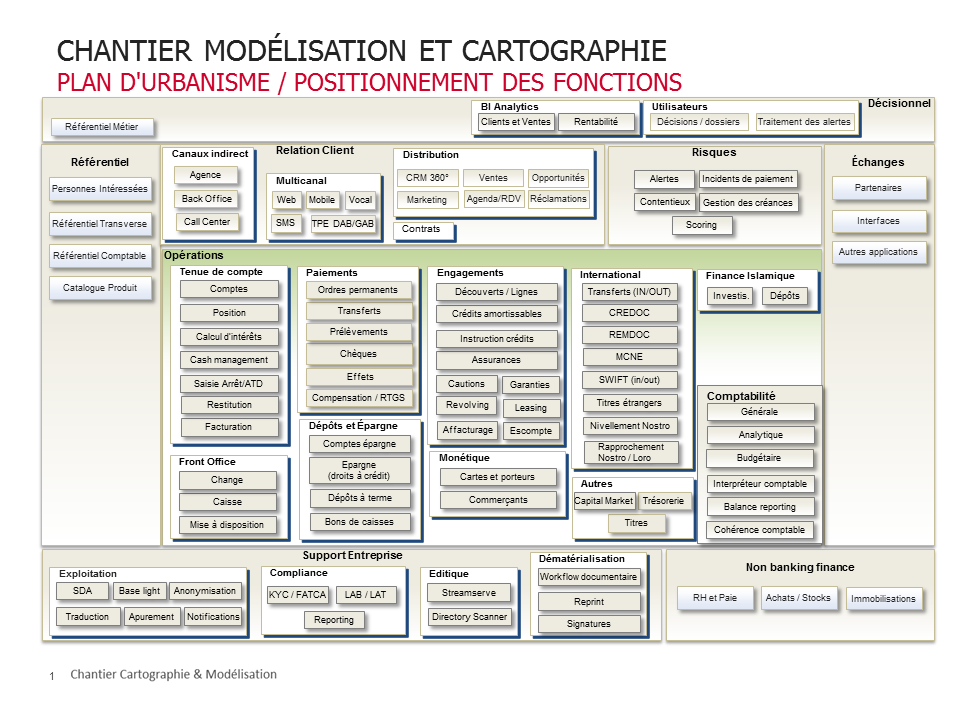
\includegraphics[scale=0.62]{images/Cartographie_fonctionnelle}
	\caption{Cartographie fonctionnelle d'\textit{Amplitude}}
	\label{fig:carto}
\end{figure}

D'un point de vue du code tel qu'il est implémenté, les sources d'une version \textit{Amplitude} comporte les répertoires suivants:

\begin{description}
	\item[BaseProg] : contient la liste des fichiers \textbf{BaseProg}. Ceux-ci répertorient les modules utilisés pour un programme donnée
	\item[base\_ref] : contient le schéma de référence \textit{Amplitude}, sert principalement à la compilation
	\item[bin] : contient la liste des sources binaires
	\item[migration] : contient la liste des scripts permettant de gérer les migrations de serveur
	\item[src] : contient les répertoires sources 4gl et \textit{per} (les écrans) organisés par module (ATTENTION: ne pas confondre module en tant que qu'entité pour l'organisation et module 4gl, c'est-à-dire les fichiers sources)
	\item[xcf] : contient la liste des services métiers génériques (SMG) disponibles. Les SMG sont des programmes utilisés par \textit{Amplitude} mais extérieur au progiciel.
	\item[xsd] : contient les fichiers \textit{xsd} nécessaires au produit.
\end{description}

Nous ne rentrerons pas dans le détail du fonctionnement de chacune des sources présentées ici, mais nous verrons davantage d'éléments sur ce qui nous servira pour le projet dans la suite du rapport (dans la \autoref{part:dev} notamment).

\chapter{Présentation du projet}

\section{Contexte}

Le projet a été lancé à la demande des architectes fonctionnels du progiciel qui effectuent des revues d'analyses. Leurs objectifs sont les suivants:

\begin{itemize}
	\item Maîtriser l’évolution du modèle de données \textit{Amplitude} pour assurer la pérennité et l’évolutivité dans le temps d’\textit{Amplitude} en urbanisant les données et en standardisant les développements,
	\item Orienter l’analyste pour qu’une solution ou un concept réutilisable soit développé(e) et rechercher s’il existe des pistes d’améliorations possibles sur la solution / le concept existant(e) et transmet les axes d’améliorations,
	\item Valider que les solutions proposées par l’analyste respectent bien les règles et principes d’architecture fonctionnelles et techniques du produit \textit{Amplitude}, et qu’elles sont conformes à la politique éditeur \textit{Amplitude Up}.
\end{itemize}

Or actuellement dans l'entreprise, aucun outil ne permet de recenser des flux entrants et sortants d'\textit{Amplitude}, d'analyser les impacts suite au développement et de visualiser la cartographie. Les architectes fonctionnels utilisent des fichiers Excels répertoriant ses informations, ce qui n'est pas la meilleure solution d'un point de vue efficacité.

Ainsi, la réalisation d’un outil de fiabilisation des informations de recensement, des analyses et de leur visualisation améliorerait la maîtrise du modèle de données \textit{Amplitude} et faciliterait donc la vie aux architectes fonctionnels, voire même aux développeurs.


\section{Expression du besoin}

Les besoins principaux demandés sont les suivants:

\begin{description}
	\item[Dictionnaire des flux, interfaces et éditions] : l'idée serait de faire un dictionnaire regroupant l'ensemble de flux entrants et sortants d'\textit{Amplitude}. Cela permettrait de gagner en efficacité lors des revues d'analyses et de solution, d'améliorer l'efficacité de l'ensemble des acteurs sur l'analyse d'impact de l'évolution et d'apporter une meilleur plus-value pour les clients.
	\item[Analyse et alerte sur les impacts développements] : avoir un aperçu des impacts que pourraient avoir la modification d'une fonction d'un module. Cela faciliterait l'analyse d'impact pour les analystes, les testeurs et les architectes, de donner une vision globale aux nouveaux arrivants et de prévenir les risques en cas d'évolution futures.
	\item[Visualisation de la cartographie] : avoir un aperçu global de la cartographie, pouvoir zoomer sur les sous-fonctions, les programmes, les tables, etc., ajouter des commentaires...
\end{description}


\section{Description des exigences}

L'outil de cartographie devrait supporter les versions d'\textit{Amplitude Up} ouvertes aux clients (version 11 et supérieur). L'outil sera interfacé avec le dictionnaire des données qui regroupe les éléments de la cartographie fonctionnelle ainsi qu'aux versions d'\textit{Amplitude} souhaitées par le biais de SVN. 

Le but du projet étant de proposer une visualisation de la cartographie, l'outil devra avoir une interface claire, lisible, qui puisse perdurer à l'avenir. Ainsi, le choix d'utiliser \textit{Angular} pour la partie front-end est venu (le fonctionnement d'\textit{Angular} est détaillé dans le \autoref{chap:angular}). Des fonctions de recherche devront être implémentées pour retrouver facilement les entités que l'on souhaite observer.

Les programmes d'\textit{Amplitude} devront être répertoriés avec, quand cela est possible, les informations suivantes:

\begin{itemize}
	\item Le nom du programme
	\item La description du programme
	\item Les champs d’application du programme : standard, spécifique adhérent, spécifique non adhérent, etc. La liste doit être paramétrable
	\item Les caractéristiques du programme : le pays, la zone géographique, le client ou groupe, etc. La liste doit être paramétrable
	\item Le type de programme : batch, transactionnel, écran (attention, plusieurs choix possibles pour un programme)
	\item Les commentaires
\end{itemize}


\section{Gestion de projet}

Le projet suivra une méthode agile pour plusieurs raisons. Tout d'abord, il s'agit d'un projet en interne visant à améliorer la productivité des personnes travaillant sur \textit{Amplitude}. Il n'y a pas d'obligation de mise en production pour un client par exemple. Ensuite, le projet sera divisé en plusieurs lots, avec un lot principal qui devrait terminer à l'issue de mon stage, et de futurs lots incluant des besoins qui n'ont pas été pris en compte dans le premier lot.  

Je serai la seule personne qui va travailler sur l'outil de cartographie à temps plein. Néanmoins, je vais être accompagné pendant toutes les étapes pour mon encadrant et par mes collègues lorsque certains problèmes bloquants se présenteront et pour la réalisation de certaines tâches plus complexes (notamment la gestion de la sécurité de l'application).


\part{Tutoriels et formations}

Cette partie sera consacrée aux différents tutoriels et formations que j'ai effectué lors des premières semaines de stage (approximativement les 3 semaines du mois d'Avril). Après avoir pris connaissance du sujet et des locaux, une phase de mise à niveau sur les outils que nous allions utiliser s'imposait. Le principe était de réaliser des tutoriels préconisés par mon encadrant (tutoriels internes à \textit{Sopra} ou sur Internet) et de réaliser des comptes-rendus (ou \textit{Proof of Concept}) sur les outils observés pour que les personnes souhaitant s'intéresser au sujet puissent avoir un support disponible. Les formations étaient portées sur trois technologies principales : \textit{Spring Boot}, \textit{Spring Data} et \textit{Angular}. Ces technologies seront détaillées dans cette partie.

Avant de rentrer dans les détails, il est important d'avoir quelques connaissances en développement au préalable, en particulier en langage Java, sur certains frameworks et sur l'outil de construction de projet \textit{Maven}. Les notions basiques de \textit{Maven} sont résumées rapidement sur le site de documentation d'Apache ici : \url{https://maven.apache.org/guides/getting-started/maven-in-five-minutes.html}.


\chapter{Spring Boot}


\textit{Spring Boot} a pour but de faciliter la création d'application utilisant \textit{Spring} en automatisant ses configurations. \textit{Spring Boot} permet par ailleurs de créer pour un projet, un exécutable unique contenant toutes les dépendances nécessaires. Les objectifs annoncés par la documentation de \textit{Spring Boot} sont les suivants : 

\begin{itemize}
	\item Proposer des solutions rapides et accessibles pour les développements \textit{Spring} ;
	\item Faciliter les configurations, même lorsque les paramètres souhaités diffèrent de ceux utilisés par défaut ;
	\item Proposer une panoplie d'options non-fonctionnelles (comme des serveurs embarqués \textit{Tomcat}, des options de sécurité, de mesures de performances, etc.) ;
	\item Aucune génération de code ni de configuration XML. 
\end{itemize}

\textit{Spring Boot} ne génère pas de code ni ne modifie les fichiers du projet. Au démarrage de l'application, \textit{Spring Boot} va dynamiquement « brancher » les composants et les configurations nécessaires au contexte du projet. Les deux principales modifications à opérer pour faire fonctionner \textit{Spring Boot} se passent sur le fichier \textit{Maven} et au travers d’annotations du framework \textit{Spring} sur les composants en action. Le détail du fonctionnement sera détaillé dans les prochaines sections. 

\textit{Spring Boot} fonctionne avec les versions Java 1.8 et supérieur. Les différentes versions des composants utilisés par \textit{Spring Boot} sont détaillés dans le guide de référence à l’adresse suivante : \url{https://docs.spring.io/spring-boot/docs/2.0.1.RELEASE/reference/htmlsingle/}.


\section{Création d'un projet avec \textit{Spring Initializr}}

Il est possible de générer un projet \textit{Spring Boot} avec toutes les dépendances que l’on souhaite \textit{Spring Initializr} à l’adresse : \url{https://start.spring.io/}. Un aperçu du site est visible sur la \autoref{fig:initializr}.

\begin{figure}
	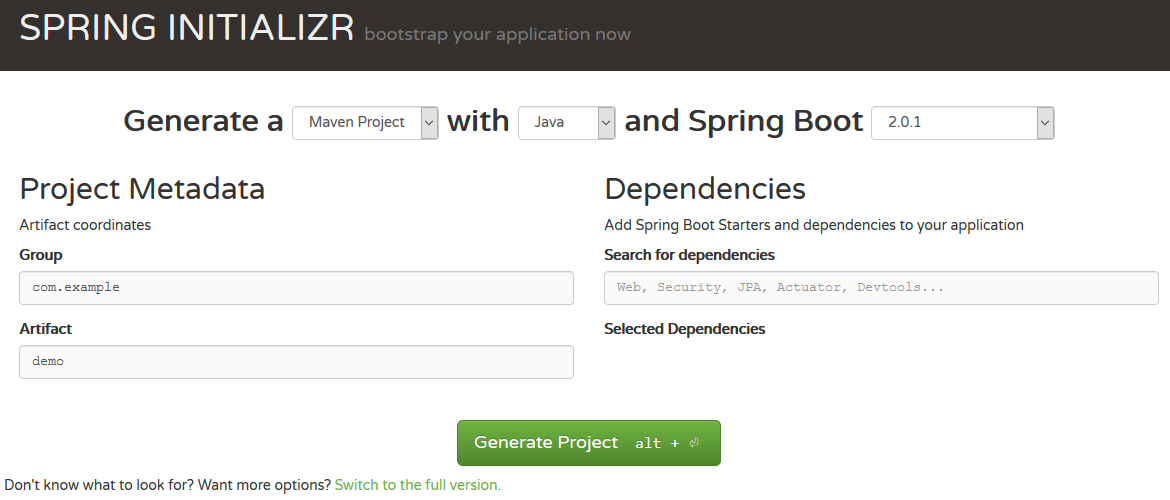
\includegraphics[scale=0.5]{images/springInitializr}
	\caption{Aperçu du site \textit{Spring Initializr}}
	\label{fig:initializr}
\end{figure}

Pour générer un projet, il suffit d’indiquer les propriétés du projet et les dépendances que l’on souhait ajouter et un modèle de projet \textit{Spring Boot} sera disponible au téléchargement. Les détails et le fonctionnement du fichier \textit{pom.xml} généré sont détaillés dans la prochaine section. 

La création d'un projet par ce biais n'est pas obligatoire, cependant dans les cas où l'on connaît par avance les principales dépendances de notre projet, cela s'avère être un gain de temps non négligeable. Le projet généré est sous forme de dossier compressé \textit{.zip} contenant la structure du projet, le fichier de construction du projet \textit{pom.xml} de \textit{Maven} avec toutes les dépendances, et les classes principales. 

\section{Utilisation avec \textit{Maven}}
\label{sec:utilisationMaven}

Pour utiliser \textit{Spring Boot} via l’outil \textit{Maven}, la solution la plus courante est de faire hériter son projet du \textit{spring-boot-starter-parent} qui contient les dépendances de bases de \textit{Spring Boot} en ajoutant cette partie au début du fichier \textit{pom.xml} :

\begin{figure}
	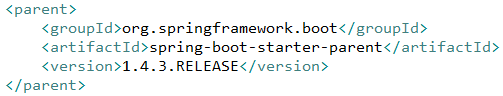
\includegraphics[scale=1]{images/parentSpringBoot}
	\caption{Extrait d'implémentation de la dépendance parent dans le \textit{pom.xml}}
	\label{fig:parentSpringBoot}
\end{figure}

Ensuite, dans la partie \textit{dependencies}, on ajoute les starters correspondant au type d’application que l’on souhaite réaliser. Les \textit{starters} sont des dépendances \textit{Maven} regroupant toutes les configurations voulues pour l’application.  Par exemple, si l'on souhaite réaliser une application web, on ajoute la dépendance \textit{spring-boot-starter-web} dans le fichier \textit{pom.xml}: 

\begin{figure}
	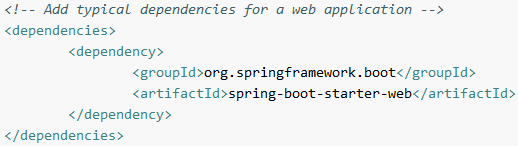
\includegraphics[scale=1]{images/dependencySpringBoot}
	\caption{Extrait d'implémentation d'une dépendance web dans le \textit{pom.xml}}
	\label{fig:dependencySpringBoot}
\end{figure}

Cela embarquera toutes les dépendances nécessaires au fonctionnement d'une application web, comme un serveur embarqué \textit{Tomcat} par exemple. Tous les starters suivent la même syntaxe : \textit{spring-boot-starter-*}, avec * le type de projet souhaité. Parmi les différents starters disponibles, voici un liste des plus intéressants pour plusieurs types de projets :

\begin{description}
	\item[spring-boot-starter] Starter central, auto-configure le support, le logs et les fichiers YAML.
	\item[spring-boot-starter-web] Utilisé pour réaliser des application web utilisant Spring MVC. Utilise Tomcat comme conteneur embarqué par défaut.
	\item[spring-boot-starter-thymeleaf] Utilisé pour les applications Web MVC avec les vues de Thymeleaf.
	\item[spring-boot-starter-test] Utilisé pour la réalisation de tests. Il implémente plusieurs bibliothèques de tests comme JUnit, Mockito, etc..
	\item[spring-boot-starter-actuator] Utilisé pour la mise en production, ajoute des fonctionnalités pour monitorer et gérer l’application. 
	\item[spring-boot-starter-jdbc] Utilisé pour JDBC avec le pool de connexion HikariCP.
	\item[spring-boot-starter-data-jpa] Utilisé pour Spring Data JPA avec Hibernate.
	\item[spring-boot-starter-security] Utilisé pour Spring Security.
\end{description}

La liste complète des starters se trouvent à l’adresse suivante : \url{https://docs.spring.io/spring-boot/docs/2.0.1.RELEASE/reference/htmlsingle/#using-boot-starter}.

Ensuite, pour empaqueter l'application dans un exécutable, il suffit de rajouter le plug-in maven dans la partie \textit{build} du fichier \textit{pom.xml} comme on peut le voir dans la \autoref{fig:buildSpringBoot}.

\begin{figure}
	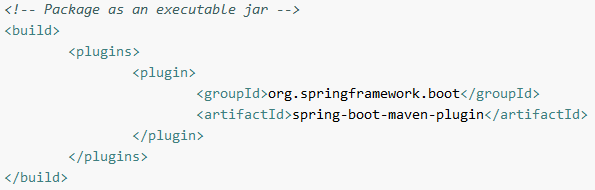
\includegraphics[scale=1]{images/buildSpringBoot}
	\caption{Implémentation du plug-in \textit{Maven}}
	\label{fig:buildSpringBoot}
\end{figure}

Il s’agit de l’essentiel des modifications à apporter dans le fichier de configuration de \textit{Maven} pour faire fonctionner une application \textit{Spring Boot}. Il est possible d’ajuster d’autres paramètres ou d’ajouter davantage de fonctionnalités. Par exemple, pour les applications web, la dépendance \textit{spring-boot-devtool} permet d’effectuer des rafraîchissements à la volée sans recompiler l’intégralité du code. 


\section{Éléments à ajouter dans le programme}
\label{sec:elementsSpringBoot}

La configuration des projets \textit{Spring Boot} nécessite l’utilisation d’annotations du framework \textit{Spring} pour définir l’architecture du projet et les interactions entre les composants. L’annotation principale à ajouter est \javacode{@SpringBootApplication}.


Cette annotation doit être placée sur la classe principale du projet et correspond à 3 annotations \textit{Spring}:
\begin{itemize}
	\item \javacode{@Configuration} qui indique que la classe est la source pour le contexte donné;
	\item \javacode{@EnableAutoConfiguration} qui indique à \textit{Spring Boot} d’ajouter les configurations définies au préalable;
	\item \javacode{@ComponentScan} qui indique à \textit{Spring} de regarder les configurations dans les autres classes du même package;
\end{itemize}

Ensuite, la méthode \textit{main()} utilise la fonction dédiée au lancement de l’application de \textit{Spring Boot} : \javacode{SpringApplication.run()}. Sur la \autoref{fig:mainSpringBoot}, un exemple de classe principale basique utilisant la fonction \javacode{run()} et l’annotation pour le lancement de \textit{Spring Boot}.

\begin{figure}
	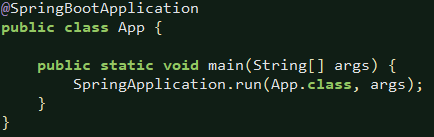
\includegraphics[scale=1]{images/mainSpringBoot}
	\caption{Fonction principale d'un projet \textit{Spring Boot}}
	\label{fig:mainSpringBoot}
\end{figure}

\textit{Spring Boot} se connecte automatiquement à la classe principale du projet. Or, il est possible qu’un projet comporte plusieurs classes principales. Pour pallier à cela, il est possible de définir la classe que l’on souhaite lancer dans le fichier \textit{pom.xml} de deux manières : soit dans la partie \textit{properties} dans une balise \textbf{<start-class>}, soit dans la partie \textit{build} dans une balise <\textbf{configuration>} comme dans la  \autoref{fig:multipleMainSpringBoot}.

\begin{figure}
	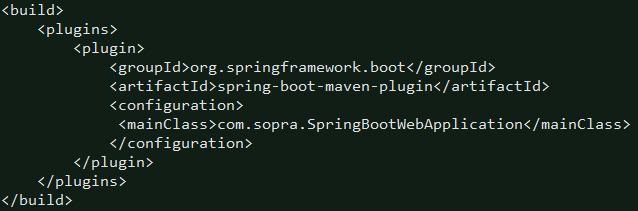
\includegraphics[scale=0.8]{images/multipleMain}
	\caption{Fichier \textit{pom.xml} en cas de multiples fonctions principales}
	\label{fig:multipleMainSpringBoot}
\end{figure}

Dans le cas où l'on souhaite réaliser des tests unitaires, on peut ajouter le starter \textit{spring-boot-starter-test} dans le fichier \textit{pom.xml}. Puis, on annote les classes de tests par \javacode{@SpringBoottest} ce qui permet de notifier à \textit{Spring Boot} que la classe annotée par la balise correspond à une classe de tests et ainsi, d'ajouter les configurations automatiques nécessaires.

\section{Exemple d'application web avec \textit{Spring Boot}}

Il existe plusieurs façons de réaliser une application Web avec Spring Boot. La dépendance permettant d’importer les principales configurations est spring-boot-starter-web qui utilise Spring MVC pour fonctionner. D’autres starters peuvent être utilisés pour certains cas, par exemple pour une application web MVC, si l’on souhaite gérer les vues avec Thymeleaf ou Mustache, la dépendance spring-boot-starter-thymeleaf ou spring-boot-starter-mustache configurera automatiquement les paramètres nécessaires. 

Par défaut, Spring Boot utilise les conteneurs Tomcat. Il est possible d’utiliser un autre conteneur que Tomcat, comme Jetty par exemple, mais il faut au préalable exclure Tomcat des dépendances du fichier pom.xml, comme sur la \autoref{fig:webBuildSpringBoot}.

\begin{figure}
	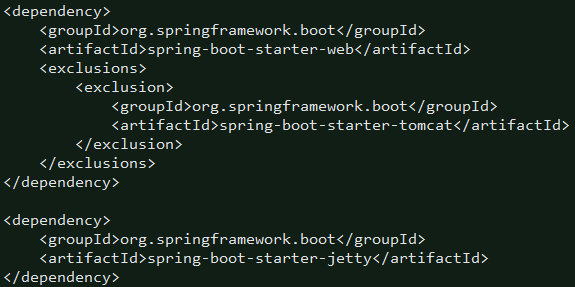
\includegraphics[scale=0.8]{images/webBuildSpringBoot}
	\caption{Fichier \textit{pom.xml} en cas de multiples fonctions principales}
	\label{fig:webBuildSpringBoot}
\end{figure}

Le port d’écoute utilisé par défaut est le 8080. Pour le modifier, plusieurs possibilités existent :

\begin{itemize}
	\item Indiquer le port souhaité dans un fichier \textit{application.properties} ou \textit{application.yml};
	\item Faire figurer dans une méthode le changement de port;
	\item Le faire figurer en ligne de commande au lancement du \textit{jar} exécutable (exemple : \javacode{java -jar -Dserver.port=8888 spring-boot-example-1.0.jar}).
\end{itemize}

Dans le cas où un port est spécifié à la fois dans le fichier \textit{application.properties} et dans le code, alors c’est le code spécifié dans le code qui sera pris en compte.

Ensuite, dans le code, il suffit d’annoter la classe main comme expliquée dans la \autoref{sec:elementsSpringBoot} et d’ajouter un contrôleur basique pour faire fonctionner le tout. 

\section{Gestion de base de données}

La gestion et la configuration d’une base de données avec \textit{Spring Boot} se fait de façon simple et automatisé. Il existe plusieurs starters permettant de gérer une base de données avec \textit{Spring Boot}, ici nous allons évoquer le fonctionnement avec JDBC, puis avec JPA et \textit{Spring data}.

Il y a principalement 3 dépendances à ajouter dans le fichier \textit{pom.xml} si l’on souhaite utiliser JDBC: \textit{spring-boot-starter} pour la configuration principale de l’application, \textit{spring-boot-starter-jdbc} pour les dépendances avec JDBC et le driver de la base de données que l’on souhaite utiliser. Comme pour les autres dépendances, \textit{spring-boot-starter-jdbc} utilise Tomcat pour gérer les connexions. Pour modifier cela, il faut d’abord exclure la dépendance Tomcat, puis ajouter celle que l’on souhaite par la suite. Par exemple, si l’on utilise une base de données Oracle et une connexion via DBCP2, les dépendances du fichier \textit{pom.xml} seront tels qu'on peut les trouver sur la \autoref{fig:bddBuild}. 

\begin{figure}
	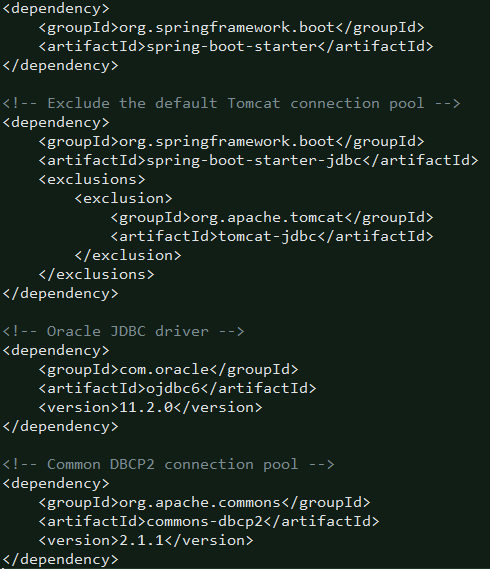
\includegraphics[scale=0.75]{images/bddPom}
	\caption{Exemple de dépendances dans le \textit{pom.xml} pour la gestion d'une base de données}
	\label{fig:bddBuild}
\end{figure}

Ensuite, les paramètres de connexions de la base de données sont indiqués dans le fichier de configuration \textit{application.properties} comme sur la \autoref{fig:bddProperties}.

\begin{figure}
	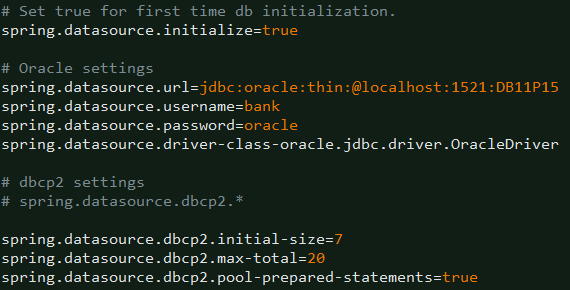
\includegraphics[scale=0.9]{images/bddProperties}
	\caption{Fichier de configuration pour l'initialisation d'une base de données}
	\label{fig:bddProperties}
\end{figure}

\textit{Spring Boot} s’occupe de l’initialisation de la base de données automatiquement. Par défaut, il va charger les scripts \textit{schema.sql} et \textit{data.sql} dans le répertoire du projet et les lancer lorsque le projet est exécuté. Le fonctionnement est différent lorsque l’on utilise Spring Data JPA. 

Pour l’utilisation avec Spring Data JPA, dans le fichier \textit{pom.xml}, on utilise la dépendance \textit{spring-boot-starter-data-jpa} à la place de \textit{spring-boot-starter-jdbc}. De la même manière, on peut modifier la connexion \textit{Tomcat} par défaut par celle de son choix. Pour l’initialisation de la base de données, en utilisant \textit{Hibernate}, il est possible de définir le fonctionnement automatique lors du lancement de l’application au travers d’une variable \textit{spring.jpa.hibernate.ddl-auto}. Cette variable peut prendre 5 valeurs qui correspondent à 5 mises en place différentes: \textit{none}, \textit{validate}, \textit{update}, \textit{create} et \textit{create-drop}. Elle peut être explicitée dans le fichier \textit{application.properties}. Si elle n’est pas définie explicitement, \textit{Spring Boot} choisira une valeur par défaut selon la base de données intégrée au projet. 

En utilisant la variable \textit{spring.jpa.hibernate.ddl-auto}, il n’est pas nécessaire d’ajouter une variable \textit{spring.datasource.initialize} étant donné que l’initialisation est gérée par la variable d’Hibernate.


\section{Déploiement d'une application \textit{Spring Boot} x \textit{Angular}}


Dans le cadre de la réalisation d’un projet multi-module, il est devenu courant de gérer une application Web avec une partie front-end qui utilise Angular pour profiter de ses facilités de développement et une partie back-end qui utilise \textit{Spring Boot} et \textit{Spring Data}, ce qui sera par ailleurs le cas pour notre projet. Se pose alors la question du déploiement d’une telle application. Plusieurs possibilités existent pour déployer ce type de projet multi-module, nous allons ici en voir 3 parmi d’autre.

\subsection{Déployer les parties séparément}

La solution la plus simple, et la meilleure pratique, est de séparer la partie front et la partie back de l’application. Cela permet d’améliorer l’évolutivité et la gestion du projet. En effet, en séparant les parties, les développements peuvent se faire en parallèle, avec une équipe dédiée au front-end et une au back-end, sans impacter l’une ou l’autre équipe. Cela permet également de réduire les temps d’indisponibilité de la plateforme, car si la partie back est indisponible, la partie front sera accessible malgré tout pour le client.

Néanmoins, pour une petite équipe, gérer deux serveurs peut s’avérer difficile et réunir les deux modules en un seul serait un avantage. Pour cela, plusieurs solutions existent, utilisant les possibilités de Maven ou de \textit{Spring Boot}, mais il faut garder à l’esprit qu’un projet \textit{Angular} n’est pas optimisé pour fonctionner avec Maven. 

\subsection{Déploiement sous forme de \textit{.war} avec \textit{Maven}}

Maven offre la possibilité d’assembler plusieurs modules en un seul. Pour cela, il faut disposer les projets dans un dossier parent et y ajoute un nouveau fichier pom.xml. Ce fichier va permettre à Maven de construire les deux projets fils avec une seul commande. Le fichier \textit{pom.xml} du dossier parent ressemblera à l’image suivante. On peut voir que le projet dispose de deux modules correspondant à la partie Spring Boot et à la partie Angular. 

\begin{figure}
	\includegraphics[scale=0.6]{images/pomParent}
	\caption{Fichier \textit{pom.xml} d'un projet multi-module}
	\label{fig:pomMultiApp}
\end{figure}

Le déploiement se fera sous la forme d’un fichier \textit{.war} qui va regrouper toutes les dépendances, les classes et les ressources de notre application web. Le fichier va se trouver dans le dossier target du module fils Spring Boot. Pour pouvoir le générer avec tous les éléments, plusieurs ajustements sont nécessaires. Tout d’abord, il faut ajouter un fichier \textit{pom.xml} au projet Angular. Comme Angular n’est pas configuré pour fonctionner avec Maven mais avec Node, le fichier pom.xml va exécuter les commandes npm install et npm build pour compiler le projet. Par défaut, les ressources compilées se trouvent dans le fichier dist de la partie Angular. 

Dans la partie back-end, la compilation Maven devra générer le fichier .war en récupérant les données compilées dans la partie Angular. Pour cela, il faut utiliser les plug-in Maven War, qui va générer le fichier, et Maven Resources, qui va copier les ressources compilées du projet Angular dans un dossier de la partie Spring Boot. Un exemple de fichiers pom.xml pour la partie Client et pour la partie Serveur est disponible sur le site \url{http://www.devglan.com/spring-boot/spring-boot-angular-deployment}.


\subsection{Déploiement sous forme de \textit{.jar} en utilisant \textit{Spring Boot}}

Il existe également la possibilité d’utiliser les fonctionnalités de Spring Boot pour déployer son application sous forme d’un unique fichier jar contenant toutes les dépendances. Pour cela, le projet doit avoir une structure similaire à celle d’un déploiement avec Maven dans la partie précédente, c’est-à-dire un projet parent avec un fichier pom.xml qui lui est propre, et les deux projets fils avec chacun un fichier pom.xml pour son propre fonctionnement.

La configuration du fichier \textit{pom.xml} du projet Angular reste le même que pour un déploiement avec un .war. La différence se fera sur la configuration de la sortie des fichiers compilés. Dans le fichier package.json, dans la partie build, il faut ajouter le chemin de sortie avec la commande suivante : \javacode{ng build -prod -output-path dist/META-INF/resources}. \textit{Spring Boot} est pré-configuré pour aller chercher les éléments statiques dans ce répertoire. Ainsi, à la création du jar, toutes les dépendances seront ajoutées.


\chapter{Spring Data}


Spring Data est un projet auxiliaire de Spring permettant de gérer plus simplement l’accès aux données, le but principal étant d’apporter une couche d’abstraction supplémentaire pour faciliter la manipulation des données qui peuvent provenir de différentes sources. Il fonctionne avec de nombreux types de bases de données, relationnel ou non, avec des frameworks de map-reduce, ainsi qu’avec des services de données basés sur le cloud. Il contient plusieurs sous-projets qui s’adaptent aux types de bases de données utilisées. 

Parmi les fonctionnalités explicitées par la documentation, on retrouve :

\begin{itemize}
	\item Un dépôt central puissant;
	\item Création de requêtes dynamiques; 
	\item Intégration Spring simple via JavaConfig ou XML;
	\item Intégration avancée avec les contrôleurs de Spring MVC;
	\item Support pour faire de l’audit (indications sur les objets, leur date de création, dernière modification, etc.);
	\item Et d’autres…
\end{itemize}

\textit{Spring Data} met à disposition de nombreux modules qui s’adaptent à la structure de gestion de données utilisée : \textit{Spring Data JPA}, \textit{Spring Data MongoDB}, \textit{Spring Data Neo4j}, etc.

\section{Fonctionnement de base de \textit{Spring Data} et de \textit{Spring Data JPA}}

Le fonctionnement de Spring Data peut être représenté sous forme de couches, avec une couche principale appelée Spring Data Commons et de multiples modules reprenant les éléments de la couche principale et qui s’adaptent à une utilisation particulière. Spring Data Commons est basé sur trois interfaces, que l’utilisateur pour étendre selon ses besoins : Repository, CrudRepository et PagingAndSortingRepository. L’interface Repository permet d’indiquer un dépôt avec un type d’objets avec lequel on travaille. L’interface CrudRepository étend l’interface Repository et ajoute des méthodes CRUD (create, read, update, delete) pour manipuler les données. Enfin, l’interface PagingAndSortingRepository étend CrudRepository et ajoute des méthodes de pagination et de tri de données.

Ensuite, Spring Data permet d’écrire des requêtes à partir de noms de méthode. Par exemple, sur la \autoref{fig:repositorySpringData}, à l’appel de la méthode \textit{findByEmailAddressAndLastName()}, \textit{Spring Data} va créer la requête qui recherche l’email et le nom de la personne automatiquement. Il n’est donc pas nécessaire de rédiger la méthode soi-même, ce qui fait une des grandes forces de l’outil. Spring Data est capable de prendre en compte des mots-clés comme And, Or, LessThan, GreaterThan, etc.. La liste complète des mots-clés est à l’adresse \url{https://docs.spring.io/spring-data/jpa/docs/2.0.6.RELEASE/reference/html/#jpa.query-methods.query-creation}.

\begin{figure}
	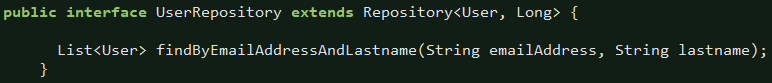
\includegraphics[scale=0.75]{images/repositorySpringData}
	\caption{Exemple de repository}
	\label{fig:repositorySpringData}
\end{figure}

Au cas où le nom de la méthode est trop long ou incommodant dans le programme, ou bien si l’on veut utiliser le nom d’une méthode en modifiant la requête qu’elle doit effectuer, il est possible d’utiliser l’annotation \javacode{@Query} pour changer le nom de la méthode à sa guise. Avant la déclaration de la méthode, cette annotation indiquera la requête que l’on souhaite réaliser lors de l’appel de la fonction.

\begin{figure}
	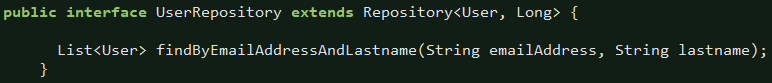
\includegraphics[scale=0.75]{images/repositorySpringData}
	\caption{Exemple de requête spécifié dans un \textit{repository}}
	\label{fig:queryRepository}
\end{figure}

Dans l’exemple de la \autoref{fig:queryRepository}, la requête associée à la méthode \textit{findByEmailAddress()} est modifiée, et est déterminée dans l’annotation \javacode{@Query}. Si la requête effectue des modifications sur les entités, il faut ajouter l’annotation \javacode{@Modifying} et éventuellement si les noms diffèrent, ajouter des annotations \javacode{@Param} pour préciser chaque entité modifiée. 

\begin{figure}
	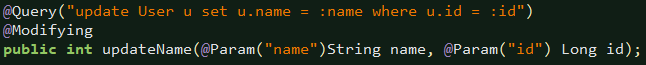
\includegraphics[scale=0.85]{images/queryModifying}
	\caption{Exemple de requête modifiée}
	\label{fig:queryModifying}
\end{figure}

Avec \textit{Spring Data JPA}, un autre repository est mise à disposition : JPARepository qui regroupe toutes les possibilités des autres repositories et ajoute des méthodes supplémentaires propres à JPA, comme \textit{flush()} pour le vidage du cache, etc.

\section{Fonctionnement de \textit{Spring Data REST}}

\textit{Spring Data Rest} est un des modules de \textit{Spring Data} permettant de faciliter la création de web-services REST. Il constitue une couche supérieure aux dépôts \textit{Spring Data} et peut exposer les données des dépôts à une application Web. Ainsi, \textit{Spring Data} nécessite une configuration avec un module de repository comme \textit{Spring Data JPA}, \textit{Spring Data MongoDB}, etc.. En général, \textit{Spring Data REST} n’ajoute pas de fonctionnalités au dépôt de données utilisé. En effet, par définition \textit{Spring Data REST} doit fonctionner avec n’importe quel projet \textit{Spring Data} qui utilise un modèle de repository.

La fonctionnalité principale de \textit{Spring Data REST} est donc d’exporter les ressources des repositories. Ainsi, en configuration standard, un dépôt \textit{PersonRepository} comme ci-dessous va exposer les ressources à l’URI /persons .

\javacode{public interface PersonRepository extends CrudRepository<Person, Long> \{ \}}

Chaque objet \textit{Person} sera également exposé selon un modèle d’URI \javacode{/persons/\{id\}}. Par défaut, les requêtes HTTP effectuées sur le web-service vont interagir avec les méthodes présentes dans CrudRepository de la manière suivante : 

\begin{itemize}
	\item Méthode \textit{create} -> requête \textbf{POST}
	\item Méthode \textit{read} -> requête \textbf{GET}
	\item Méthode \textit{update} -> requête \textbf{PUT}
	\item Méthode \textit{delete} -> requête \textbf{DELETE}
\end{itemize}

Si l’on souhaite modifier les liens sur lesquelles vont être exportés les ressources, il est possible d’ajouter une annotation \javacode{@RepositoryRestResource} avant la déclaration de l’interface.

\begin{figure}
	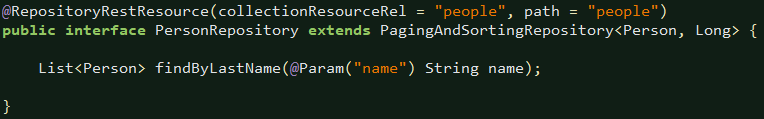
\includegraphics[scale=0.75]{images/repositoryRESTResource}
	\caption{Exposition REST d'un \textit{repository}}
	\label{fig:repositoryRESTResource}
\end{figure}

Dans l’exemple \autoref{fig:repositoryRESTResource}, les objets \textit{Person} seront exportés sur l’URI \javacode{/people} et plus sur l’URI \javacode{/persons} comme c’était par défaut. L’option \textit{collectionResourceRel} détermine la valeur à utiliser lors de la génération des liens vers les ressources et l’option \textit{path} détermine le chemin vers lequel la ressource sera exportée. 

\textit{Spring Data Rest} ajoute aussi des liens additionnels permettant de naviguer entre les enregistrements. Ces liens sont définis par les méthodes présentes dans le repository de la ressource que l’on recherche. Dans l’exemple précédent, une méthode \textit{findByLastName()} était présente. Ainsi, il est possible de rechercher les personnes par leur nom de famille. Toutes les méthodes de recherche d’un repository sont accessibles avec l’URL \javacode{/people/search}. La syntaxe pour effectuer une recherche sur les noms de famille comme indiquer dans l’exemple serait la suivante : \url{http://localhost:8080/people/search/findByLastName?name=Johnson}. Le résultat de cette recherche donnera toutes les personnes ayant pour nom de famille : Johnson. Les résultats des recherches sont disposés au format JSON. 

\section{Configuration avec \textit{Spring Boot} et \textit{Spring Data JPA}}

L’interfaçage entre \textit{Spring Boot}, \textit{Spring Data JPA} et \textit{Spring Data REST} se fait de façon très simple et automatisé. \textit{Spring Boot} utilise \textit{Spring Data JPA} pour créer une implémentation des dépôts et les configurer via une base de données utilisant JPA. \textit{Spring Data REST} va créer les contrôleurs \textit{Spring MVC}, les convertisseurs JSON et les autres éléments nécessaires pour obtenir un front-end respectant les règles REST. \textit{Spring Boot} va ensuite relier les composants du front-end avec les données de JPA de façon automatique. 

Pour lancer un projet utilisant \textit{Spring Boot}, \textit{Spring Data JPA} et \textit{Spring Data REST}, il faut ajouter les deux dépendances \textit{spring-boot-starter-data-jpa} et \textit{spring-boot-starter-data-rest} au fichier \textit{pom.xml} comme évoqué dans la \autoref{sec:utilisationMaven}.


\chapter{Angular}
\label{chap:angular}

\textit{Angular} est un framework open-source basé sur le langage \textit{TypeScript} permettant de réaliser des applications web. Il a été initié par Google en 2016 sous la forme d’un autre framework appelé \textit{AngularJS}, basé sur \textit{JavaScript}. Il a été totalement refait par les mêmes équipes pour créer Angular tel qu’on le connaît aujourd'hui. Il est néanmoins nécessaire d’être vigilant lors de la recherche d’informations sur la version d’Angular utilisée, car \textit{AngularJS}, la version 1 d’Angular, est toujours maintenu et utilisé par certains sites. La version stable d’Angular la plus récente est la version 5, cependant une nouvelle version d’Angular sort environ tous les 6 mois. La version 6 est sortie courant Avril 2018 mais n’est pas encore stable.

L’objectif d’Angular est de faciliter la réalisation d’applications web en automatisant certaines parties et en permettant d’effectuer des animations complexes avec très peu de lignes de code. Les applications Angular sont destinées à fonctionner sur les navigateurs Internet récents (Chrome, Firefox, …) et sont adaptées pour le cross-platform (fonctionner à la fois sur Desktop et sur Mobile). Le framework propose des facilités de développement comme par exemple, la compilation et la génération automatique du code permettant de voir en direct les modifications apportées. La gestion des tests unitaires est également facilitée avec le runner Karma qui permet de voir les résultats de tests directement sur le navigateur et pouvoir modifier à la volée les tests.

\section{Installations nécessaires}

\subsection{\textit{Node.js}, \textit{npm} et \textit{Angular CLI}}

Avant de pouvoir créer un projet, il est nécessaire d’installer plusieurs éléments. Tout d’abord \textit{Node.js}, une plate-forme logicielle en JavaScript permettant d’utiliser de nombreuses bibliothèques en ligne de commande. Les fichiers d’installation de \textit{Node.js} se trouvent à l’adresse \url{https://nodejs.org/en/download/}. L’installation de \textit{Node.js} inclut le gestionnaire de package \textit{npm} qui permet d’installer des applications \textit{Node.j}s à partir du dépôt \textit{npm}. L’application se lance depuis une invite de commande, il est possible de vérifier si l’installation s’est faite correctement avec la commande \javacode{npm -v} sur \textit{Windows} qui indique la version de \textit{npm}. 

Ensuite, la méthode la plus simple pour manipuler un projet \textit{Angular} est d’utiliser \textit{Angular CLI}. Il s’agit d’un outil en ligne de commande permettant de créer un projet, d’ajouter des fichiers et d’exécuter des tâches comme l’exécution, le déploiement ou le test d’une application web. L’installation d'\textit{Angular CLI} se fait avec \textit{npm} avec la commande : \javacode{npm install -g @angular/cli}.

\subsection{Quelques IDE intéressants pour le développement \textit{Angular}}

Il existe de nombreux IDE adaptés pour le développement sous \textit{Angular}. Parmi ces IDE, 3 d’entre eux semblent se démarquer des autres : \textit{Angular IDE}, \textit{WebStorm} et l’éditeur en ligne \textit{Stackblitz}.

\subsubsection{Angular IDE}

\textit{Angular IDE} est un éditeur gratuit produit par \textit{Genuitec} optimisé pour le développement \textit{Angular}. Il a la particularité d’être disponible à la fois en version standalone mais aussi sous forme de plug-in pour \textit{Eclipse} disponible sur le marketplace. Les téléchargements sont disponibles ici : \url{https://www.genuitec.com/products/angular-ide/}. 

\subsubsection{WebStorm}

WebStorm est l’éditeur faisant parti de la suite produite par Jetbrains avec IntelliJ IDEA, PyCharm et d’autres. C’est un des éditeurs les plus populaires, néanmoins il nécessite l’achat d’une licence commerciale pour l’utilisation. Il apport des fonctionnalités intéressantes comme l’auto-sauvegarde des fichiers, permettant avec Angular de voir en direct les modifications apportées au programme sans avoir à sauvegarder manuellement ses fichiers. 

\subsubsection{Éditeur en ligne: \textit{Stackblitz}}

Stackblitz est un éditeur en ligne adapté à divers types de projets Web. Il comporte les fonctionnalités basiques des IDE locaux intégré directement sur navigateur. Le projet est généré à la volée et on peut voir les modifications en direct sur la même fenêtre. Trois panneaux composent l’interface : un avec l’arborescence, un avec l’éditeur et un autre avec l’émulation du projet. 

Un des avantages de Stackblitz par rapport aux éditeurs locaux est de permettre à plusieurs personnes d’éditer un projet en même temps, à la manière de ce que propose Google Drive. Il est possible de partager le projet entier ou bien uniquement la fenêtre d’affichage. Les projets créés sur Stackblitz peuvent être téléchargés sous forme de dossier compressé. 

\section{Structure d'un projet \textit{Angular}}

Un projet \textit{Angular} est basé sur deux concepts : les modules et les composants. La construction d’une application \textit{Angular} se fait à partir des modules, qui donne un contexte pour la compilation des composants. Un module collecte les différentes fonctions qui lui sont liées pour l’assemblage du projet. Une application Angular est toujours composée d’au moins un module, appelé root module qui assemblent les éléments nécessaires au lancement du programme. 

Les composants définissent les vues de l’application, et une application est constituée d’au moins un composant appelé root component. Chaque composant est définie par au minimum 2 fichier : un fichier HTML qui va définir le modèle d’affichage du composant et un fichier TypeScript avec les données et les fonctions associées à la classe. À ces deux fichiers, on peut en rajouter deux autres qui ne sont pas obligatoires pour le fonctionnement d’un projet : un fichier CSS pour associer un style au template HTML et un autre fichier TypeScript, distingué par une extension \textit{.spec.ts}, qui définit des tests unitaires.

Les modules et composants de base sont générés lors de la création du projet et donne une arborescence comme on peut le voir sur la \autoref{fig:arborescenceAngular} dans le dossier \textit{/src}.

\begin{figure}
	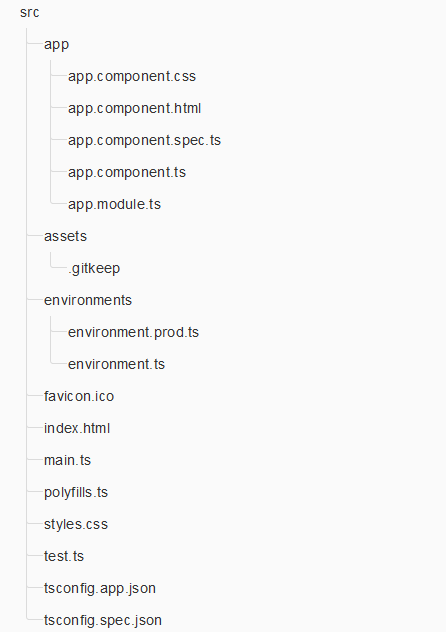
\includegraphics[scale=0.85]{images/arborescenceSrc}
	\caption{Arborescence d'un projet \textit{Angular}}
	\label{fig:arborescenceAngular}
\end{figure}

Ici, le module et le composant par défaut sont disposés dans le dossier app. Les autres fichiers sont détaillés dans la documentation à l’adresse : \url{https://angular.io/guide/quickstart#the-src-folder}.

Le dossier \textit{src} fait partie des nombreux autres éléments générés à la création d’un projet \textit{Angular} avec \textit{Angular CLI}. On retrouve par exemple un dossier \textit{node\_module} qui comportent tous les modules externes listés dans le fichier \textit{package.json} présent à la racine du projet. Les autres fichiers sont présentés dans la documentation à l’adresse \url{https://angular.io/guide/quickstart#the-root-folder}.


\section{Gestion des styles: \textit{Bootstrap} et \textit{PrimeNG}}

Il est possible d’appliquer des styles sur les différents composants que l’on souhaite avec les fichiers CSS. Cependant, réaliser un thème cohérent CSS de A à Z est très chronophage. Il existe plusieurs frameworks permettant d’appliquer des thèmes et de réaliser des animations responsives de manière très simple. Par défaut, un projet \textit{Angular} dispose d’une feuille de style de base appelée \textit{styles.css} qui est vide. Il permet d’appliquer des styles sur l’ensemble de l’application. Il est possible de changer la feuille de style par défaut appliquée au projet ou bien d’en ajouter plusieurs dans le fichier \textit{.angular-cli.json} au niveau de l’option \textit{styles}.

\begin{figure}
	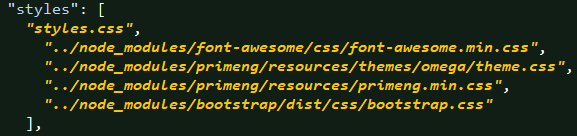
\includegraphics[scale=0.85]{images/styles_angular-cli}
	\caption{Sélection des styles en Angular}
	\label{fig:stylesAngular}
\end{figure}

Parmi les nombreux frameworks existants, en voici deux parmi les plus populaires pour le développement Web actuellement : \textit{Bootstrap} et \textit{PrimeNG}.

\subsection{\textit{Bootstrap}}

\textit{Bootstrap} est une bibliothèque gratuite et open-source permettant de concevoir des applications et des sites web. Utilisée sur un projet, elle permet d’ajouter des éléments responsives, comme des boutons, des panneaux dynamiques et bien d’autres facilement. La bibliothèque est compatible avec la majorité des navigateurs internet sur PC de bureau ainsi que sur mobile. Voici un visuel de ce que peut donner une application avec \textit{Bootstrap}. 

\begin{figure}
	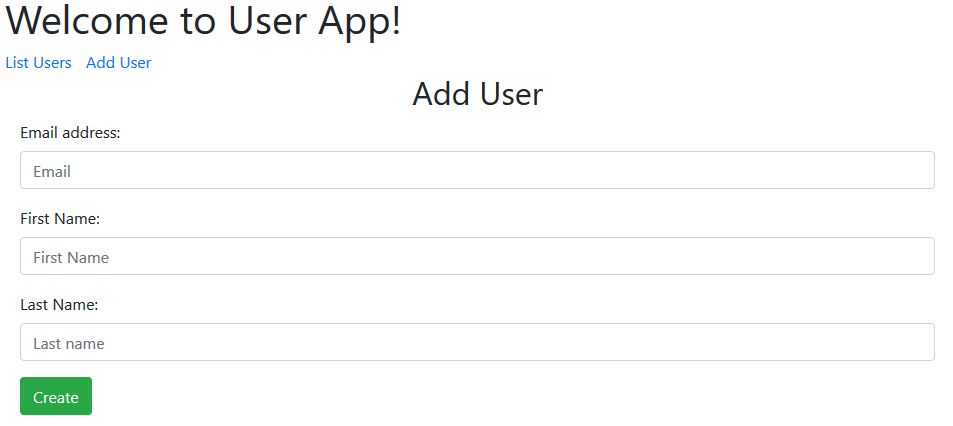
\includegraphics[scale=0.6]{images/bootstrap_exemple}
	\caption{Exemple de page formatée avec \textit{Bootstrap}}
	\label{fig:boostrapExemple}
\end{figure}

Pour utiliser le template Bootstrap avec Angular, il suffit de l’installer en utilisant la commande npm install bootstrap, puis d’ajouter la feuille de style dans le fichier .angular-cli.json comme sur l’image vu auparavant. Ensuite, l’appel des classes se fait via les fichiers HTML relatifs au composant Angular que l’on souhaite voir impacter. La documentation pour pouvoir utiliser pleinement les capacités de Bootstrap se trouve à l’adresse : \url{https://getbootstrap.com/docs/4.1/getting-started/introduction/}.

\subsection{\textit{PrimeNG}}

PrimeNG est une bibliothèque adaptée pour Angular permettant d’ajouter toute sorte de composants et de widgets pour les applications Web. PrimeNG est gratuit, open-source et peut être utilisé de façon complémentaire à Bootstrap. Parmi les composants disponibles, il y a divers types de boutons, de graphiques, de panneaux, compatibles avec différents thèmes. Le site de PrimeNG (\url{https://www.primefaces.org/primeng/#/}) permet de voir directement toutes les possibilités offertes par le framework. 

Pour l’utiliser sur un projet, il faut tout d’abord l’installer avec la commande \javacode{npm install primeng --save}. Une fois installée, de la même manière que pour Bootstrap, il faut ajouter les styles que l’on souhaite dans le fichier \textit{.angular-cli.json}. Par exemple, pour appliquer le thème Omega de PrimeNG, il faut ajouter les styles comme sur la \autoref{fig:stylesPrimeNG}. 

\begin{figure}
	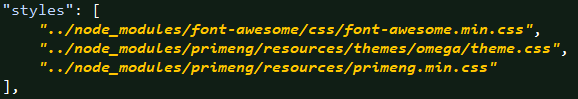
\includegraphics[scale=0.8]{images/styles_primeng}
	\caption{Exemple de styles utilisant \textit{PrimeNG}}
	\label{fig:stylesPrimeNG}
\end{figure}

Ensuite, pour ajouter un module en particulier, par exemple si l’on souhaite ajouter un tableau, il faut importer le module dans le root module de l’application et ensuite, suivre les instructions du site PrimeNG pour voir la balise HTML à utiliser pour ce module. Pour ajouter notre tableau par exemple, le fichier HTML ressemblera à \autoref{fig:primeNGHTML}, avec des balises \textit{p-table} pour représenter le tableau en question.

\begin{figure}
	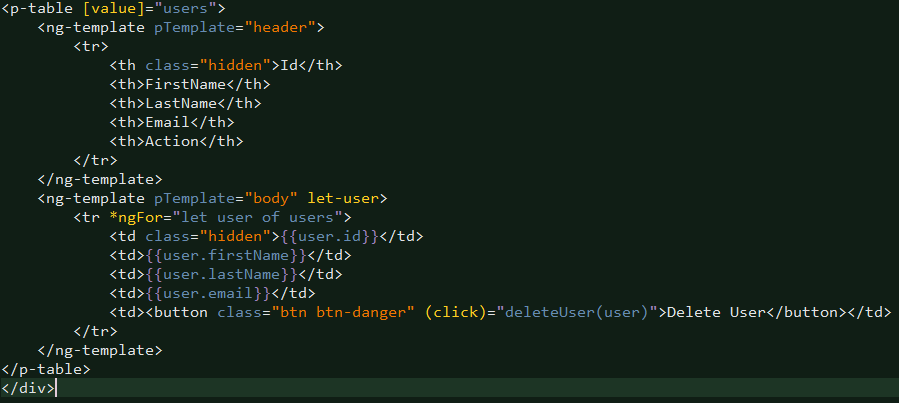
\includegraphics[scale=0.65]{images/primeng_html}
	\caption{Implémentation HTML utilisant \textit{PrimeNG}}
	\label{fig:primeNGHTML}
\end{figure}


\part{Modélisation de l'outil et chiffrage du projet}

Cette partie retrace mes activités dans l'entreprise de fin Avril jusqu'au début du mois de juin. L'essentiel du travail effectué était consacré à la modélisation de l'outil, aux spécifications et au chiffrage des phases de développement du projet.  

\chapter{Modélisation UML}

L'aboutissement de la modélisation finale a demandé beaucoup d'échanges au préalable entre les architectes fonctionnels et les personnes travaillant sur l'outil, c'est-à-dire mon encadrant et moi. Des phases de recherche pour comprendre le fonctionnement d'\textit{Amplitude} afin de trouver les meilleurs méthodes pour récupérer la cartographie étaient nécessaires. 

À l'issue des réflexions, nous avons pu aboutir à plusieurs diagrammes: l'un représentant les entités que nous allons manipuler pour créer notre cartographie, et les autres représentant des diagrammes d'activités qui correspondent à l'alimentation de notre base de données.


\section{Diagramme d'entité}

On peut séparer le diagramme en deux parties distinctes: d'un côté, ce qu'on peut appeler la cartographie technique représentant les programmes et leurs implémentations; et de l'autre, la cartographie fonctionnelle qui représente les entités tels qu'elles figurent dans le dictionnaire des données.

Coté cartographie technique, on retrouve principalement les éléments suivants : Programme, Module\_4GL, Fonction technique (qui sont les fonctions au sens développeur du terme), Fichier d'échange (qui représentent les différents flux de communication). La \autoref{fig:cartoTech} montre un extrait de cette partie du diagramme.

\begin{figure}
	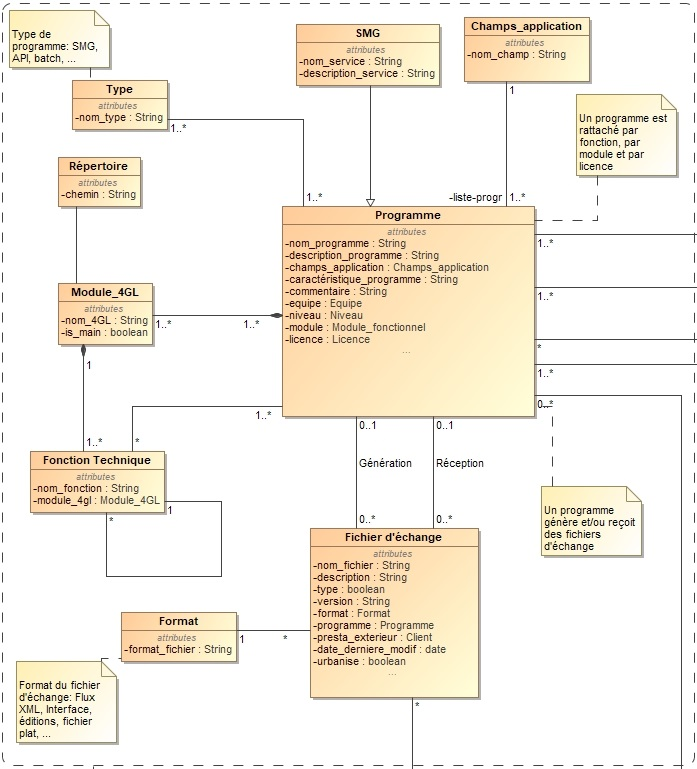
\includegraphics[scale=0.6]{images/diagCarto}
	\caption{Extrait de la partie Cartographie Technique du diagramme d'entité}
	\label{fig:cartoTech}
\end{figure}

On peut remarquer que les programmes sont les éléments qui lient la plupart des entités entre eux. En effet, un programme est composé de plusieurs modules 4GL, qui contiennent eux-même diverses fonctions. De plus, un programme peut générer ou recevoir des fichiers d'échange. En effet, un programme a un ou plusieurs types (si c'est un programme batch avec écran ou non) et peut être un Service Métiers Générique (SMG). 

Côté Cartographie fonctionnelle en revanche, on conserve la structure des dictionnaires des données, c'est-à-dire avec plusieurs niveaux de hiérarchie (domaine, fonction, sous-fonction, objet métier) liés aux tables de la base de données, puis qui seront reliés aux programmes de la cartographie technique. 

L'intégralité du diagramme, pour mieux comprendre les liaisons et la structure des entités de notre cartographie, se trouve en \autoref{ann:diagClasse}.

\section{Diagramme d'activité}

Les diagrammes d'activité représentent les agissements au cours du temps d'un processus. Ici, ils vont permettre d'avoir une vision sur les méthodes à implémenter pour le développement. La \autoref{fig:diagActivite} représente l'alimentation de notre base de données étape par étape. Il s'agit ici du schéma tel que penser au mois de mai. Plusieurs modifications ont été opérées mais l'essentiel de la structure est présente. 

\begin{figure}
	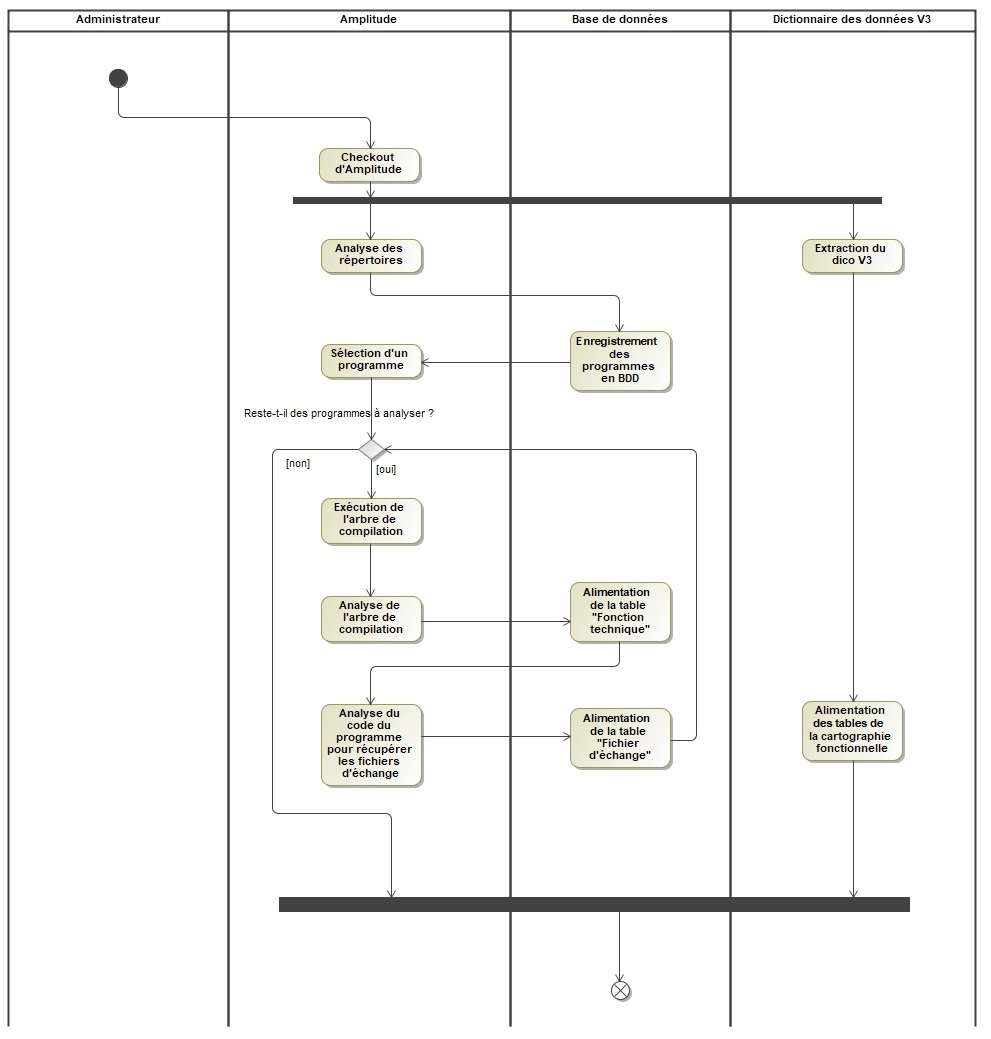
\includegraphics[scale=0.45]{images/Alimentation_initiale}
	\caption{Diagramme d'activité de l'alimentation des éléments de la cartographie}
	\label{fig:diagActivite}
\end{figure}

Le point de départ du processus d'alimentation est la récupération d'une version d'\textit{Amplitude} qui se fait par le biais de SVN, un outil de versioning. Effectuer un \textit{checkout} comme on le voit sur le diagramme signifie récupérer les sources versionnées pour pouvoir les exploiter plus facilement.

Ensuite, le processus est divisé en deux parties avec d'un côté, la récupération de la cartographie technique et de l'autre, l'extraction du dictionnaire de données V3 pour la cartographie fonctionnelle. L'idée d'un premier temps était d'enregistrer tous les programmes d'\textit{Amplitude}, puis d'analyser chacun d'entre eux pour récupérer les modules, les fonctions et les autres informations dont on a besoin, comme on peut le voir sur la \autoref{fig:diagActivite}. Ce principe n'a pas été conservé dans l'implémentation finale car il ne permettait pas de voir des fonctions ou des modules qui sont présents sur \textit{Amplitude} mais qui ne sont pas utilisés par des programmes. Ainsi, la solution que nous avons adoptée est une récupération complète des programmes, de modules et des fonctions séparément, puis une association des composants entre eux. Ce qui permet ainsi de voir l'intégralité des éléments composant \textit{Amplitude} et de distinguer les fonctions non utilisées. 

La récupération du dictionnaire des données pour la cartographie fonctionnelle se fera en réalité de manière plus simple que sur le diagramme d'activité. En effet, nous avons eu l'autorisation d'accès aux éléments de la base de données du dictionnaire de données. Ainsi, nous aurons la possibilité de les exposer en REST facilement pour les afficher par la suite. 

\chapter{Spécifications de l'outil de cartographie}

Ce chapitre sera consacré aux étapes de développement à mettre en pour réaliser l’outil de cartographie. On distinguera deux parties distinctes sur le projet: une partie \textit{back-end} avec les implémentations \textit{Java} et \textit{Spring} qui va comporter les fonctions d’analyse et de gestion des données d’Amplitude, et une autre côté \textit{front-end} avec les composants \textit{Angular} qui va gérer les affichages et les interfaces utilisateurs.

Après un premier chiffrage, nous avons pu remarquer que le temps nécessaire à la finalisation de l'outil sera supérieur à mon temps de stage restant. Ainsi, nous avons décidé de nous focaliser davantage sur la partie \textit{back-end} du projet. Les spécifications sont donc bien plus détaillées pour cette partie que pour le \textit{front-end}.

La partie \textit{back-end} de l’application regroupe les éléments de gestion des données présentes dans \textit{Amplitude}. L’outil devra tenir compte des programmes d’Amplitude, des modules 4GL présents dans l’arborescence, des fonctions composant ces modules, et plus généralement des éléments présents dans le diagramme de classe. Le modèle de données pour l’outil sera réalisé avec \textit{Spring Data}, qui permet un interfaçage automatique entre le code source en Java et le gestionnaire de base de données configuré (dans notre cas, Oracle). Une fois le modèle réalisé, nous avons songé à faire séparer le processus d'alimentation en deux: l’alimentation initiale des tables de notre modèle dans un premier temps et la mise à jour régulière des éléments de la base dans un second. Au final, la séparation des processus d'alimentation n'est pas nécessaire, et un unique job prenant en compte les deux cas de figure suffit.

La partie front-end de l’outil sera développée sous Angular et suivra une architecture REST. Les écrans devront être à même de récupérer les données exposées par la partie back-end. L’objectif des écrans est de donner un aperçu général de la cartographie. Un panneau de recherche des données devra permettre de retrouver les informations que l’on souhaite le plus simplement possible. 


\section{Création du modèle}

L’architecture du back-end sera divisée en deux parties principales : une partie cartographie fonctionnelle et une partie cartographie technique. La cartographie fonctionnelle correspond aux entités définies à partir du dictionnaire des données. Pour le moment, l’outil ira chercher directement les informations dans la base de données du dictionnaire et les exposera en REST à la partie \textit{front-end}. Ce n'est pas une méthode qui sera fiable à long terme car avoir un accès direct une base de données peut provoquer des problèmes de sécurité. Cependant, étant donné que la base de données du dictionnaire est temporaire avant une future évolution sur une autre technologie, nous avons opté pour cette solution en envisageant les possibilités avec les futures évolutions. La partie cartographie technique regroupera les analyses et les méthodes liées aux programmes et aux modules d’Amplitude. 


\section{Alimentation de la base}

Plusieurs étapes sont nécessaires afin de récupérer l'intégralité des informations nécessaire à la cartographie: la création des programmes en base, la création des modules 4GL, la création des fonctions techniques, l'association des modules 4Gl et des programmes, l'association des fonctions et des programmes, l'extraction du dictionnaire des programmes et la récupération des SMG.

Auparavant, il sera nécessaire de faire interagir le projet avec les versions d'\textit{Amplitude} en utilisant l'outil de gestion de version SVN. Ainsi, pour chaque version d’Amplitude que l’on souhaite étudier, il faudra effectuer un \textit{checkout} d’Amplitude. C’est à partir des \textit{working copy} récupérées que l’on va effectuer les analyses et les créations d’entités en base. Il sera nécessaire par la suite d’effectuer des \textit{update} des versions lors des alimentations régulières pour observer les différences et mettre à jour les versions. 

\subsection{Création des programmes en base}

La première phase de l’alimentation de la base est la création des programmes dans la base de données. La récupération des programmes se fait à partir du dossier contenant les \textit{BaseProg} (voir la \autoref{sec:architectureAmplitude} pour voir l'architecture d'\textit{Amplitude}). Ceux-ci vont nous permettre de récupérer plusieurs données qui nous intéressent : le nom des programmes, leur type quand celui-ci est indiqué et certaines caractéristiques comme le client ou la zone géographique quand elles sont disponibles. Ces données peuvent être récupérées d’après les noms des \textit{BaseProg} qui respectent la convention de nommage suivante : \javacode{module.type.nom_programme}

Dans certains cas, on retrouve le nommage suivant, ajoutant des caractéristiques: \javacode{module.caractéristique.type.nom_programme}. 

Ici, l’objectif sera de lister les fichiers de \textit{BaseProg}, de parser chaque résultat en conservant les données que l’on souhaite, puis de créer les requêtes pour alimenter notre base. 

\subsection{Création des modules 4GL en base}

Une fois les programmes enregistrés, l’étape suivante est l’alimentation des modules 4GL en base. La récupération des modules 4GL se fait en parcourant l’arborescence des fichiers sources d’Amplitude. Pour chaque dossier de l’arborescence, on liste les modules présents et on conserve en base les noms des fichiers avec leur répertoire d’origine. 


\subsection{Création des fonctions techniques en base}


Plusieurs solutions sont possibles pour récupérer les fonctions techniques. Tout d’abord, on appelle fonctions techniques, les fonctions définies dans les modules 4GL. La méthode brute pour les récupérer serait donc de parser l’intégralité des fichiers sources pour y retrouver les fonctions définies. Cependant, il existe un outil en Python permettant de retrouver les fonctions appelées dans un programme : \textit{check\_func\_xml.py}. L’idée est donc de modifier ce script afin de retrouver les fonctions définies par module 4GL. Les modifications à effectuer devront permettre de sortir un flux texte exploitable par la suite dans le programme Java avec les indications suivantes : nom de la fonction, module 4GL où elle est définie et la liste des fonctions appelées par cette fonction. Ces informations devront être ensuite conservées en base avec Spring Data. 


\subsection{Association des modules 4GL et des programmes}

À ce stade, les modules 4GL et les programmes ont été enregistrés en base. L’association des modules 4GL et des programmes se fera en utilisant le script Python \textit{l4gl.py} qui affiche la liste des modules présents dans le baseprog d’un programme. À partir de cette liste, on associe le programme sélectionné aux modules affichés suite à l’exécution du script python. Parmi ces modules, on retrouve un module portant le même nom que le programme : le module principal du programme. Cette information sera à conserver en base. 


\subsection{Association des fonctions et des programmes}

L’association des modules et des programmes se fera en utilisant le même script que pour la création des programmes en base : \textit{check\_func\_xml.py}. Pour rappel, ce programme permet d’afficher les fonctions appelées par un programme donnée. Dans notre cas, il suffit d’appeler le script pour chaque programme et d’associer les fonctions affichées avec le programme. Un modification du code Python sera nécessaire pour afficher une sortie qui correspond à notre besoin.


\subsection{Extraction du dictionnaire des programmes}

L’utilisation des données du dictionnaire des programmes va nous permettre d’ajouter des informations supplémentaires aux programmes enregistrés dans notre base et aussi d’y ajouter les modules fonctionnels. Le dictionnaire des programmes se présente sous un fichier Excel avec deux feuilles de calcul : la première décrivant la liste des programmes avec leurs descriptions, leurs modules fonctionnels associés et d’autres informations, et la seconde lisant les modules fonctionnels ainsi que leur représentation sous forme de code à 3 caractères. L’objectif pour nous sera de parcourir la liste des modules et de les enregistrer en base dans un premier temps, puis, pour chaque programme du dictionnaire, on enregistre la description associée. 


\subsection{Récupération des SMG}

Les SMG sont des programmes particuliers que l’on peut retrouver avec le type webservice. Les SMG ont néanmoins un autre nom qui désigne leur action (exemple d’un SMG: \textit{createAccount}). La récupération de ces informations se fera à partir des fichiers xcf dans l’arborescence d’Amplitude. L’objectif sera de lister les fichiers xcf, de garder en mémoire les noms de fichier, et de parser chaque fichier xcf pour récupérer le nom du programme associé. 

D’autres données concernant les SMG sont disponibles dans le dictionnaire des SMG. Il s’agit d’un fichier Excel similaire au dictionnaire des programmes qui va nous permettre d’ajouter des informations complémentaires, notamment la description du SMG. 


\chapter{Chiffrage du projet}

Une fois les différentes étapes de développement posées, nous avons pu effectué un chiffrage du projet avec le nombre de jours attribué à chaque tâche ce qui va nous permettre d'avoir une idée sur la complexité de certaines mises en place.

\begin{longtable}{|L{12cm}|r|}
	\hline 
	\textbf{Tâches}	& \textbf{Nombre de jours} \\ 
	\hline
	\hline 
	\textbf{Architecture du projet} &  \\ 
	Partie Modèle	& 1 \\
	Partie View 	& 1 \\ 
	\hline 
	\textbf{Back-end}	&  \\ 
	Création du modèle : & 10 \\
	~~\llap{\textbullet}~~ tables + entities + dao + services avec Spring Data &  \\ 
	\hline 
	\textbf{Alimentation}	&  \\ 
	Création des programmes en base : & 3 \\
	~~\llap{\textbullet}~~ Récupération de la liste des programmes dans le BaseProg &  \\ 
	~~\llap{\textbullet}~~ Parsing des résultats (récupération du nom, du type, éventuellement des caracs pour certains programmes) &  \\ 
	~~\llap{\textbullet}~~ Alimentation de la table &  \\ 
	Création des modules 4gl en base : & 2 \\
	~~\llap{\textbullet}~~ Parcours de l'arborescence d'Amplitude &  \\ 
	~~\llap{\textbullet}~~ Alimentation de la table &  \\ 
	Création des fonctions techniques en base : & 2 \\
	~~\llap{\textbullet}~~ Modification du script \textit{check\_func\_xml.py} & 3 \\ 
	~~\llap{\textbullet}~~ Appel du script python et lecture du résultat & 2 \\ 
	~~\llap{\textbullet}~~ Création des fonction techniques & 2 \\ 
	~~\llap{\textbullet}~~ Liste des fonctions appelées par la fonction sélectionnée avec alimentation & 2 \\ 
	Association des modules 4gl et des programmes : & \\
	~~\llap{\textbullet}~~ Appel de \textit{l4gl.py} et lecture du résultat & 2 \\ 
	~~\llap{\textbullet}~~ Alimentation & 2 \\ 
	~~\llap{\textbullet}~~ Détermination du module 4gl principal & 1 \\
	Association des fonctions et des programmes : & \\
	~~\llap{\textbullet}~~ Modification du script \textit{check\_func\_xml.py} & 1 \\ 
	~~\llap{\textbullet}~~ Appel du script & 2 \\ 
	~~\llap{\textbullet}~~ Alimentation de la base & 2 \\ 
	Extraction du dictionnaire des programmes : & \\
	~~\llap{\textbullet}~~ Lecture du fichier Excel & 3 \\ 
	~~\llap{\textbullet}~~ Alimentation de la base & 2 \\ 
	Récupération des SMG : & \\
	~~\llap{\textbullet}~~ Lecture du XCF & 1 \\ 
	~~\llap{\textbullet}~~ Parse du fichier XCF & 2 \\ 
	~~\llap{\textbullet}~~ Alimentation & 1 \\ 
	~~\llap{\textbullet}~~ Lecture du fichier Excel pour alimentation & 2 \\ 
	Implémentation des connexions SVN & 2 \\
	\hline 
	Création du job	& 6 \\ 
	\hline 
	\textbf{Front End} &  \\ 
	Écrans & 20 \\
	\hline 
	\caption{Chiffrage des phases de développement de l'outil de cartographie }
\end{longtable} 


Au total, le nombre de jours attribués pour finaliser l'outil est de 75, ce qui sera trop long par rapport à mon temps de stage restant. Selon nos comptes, à l'issue de mon stage, la partie \textit{back-end} de l'application sera terminée, ce qui ne sera pas le cas pour la partie \textit{front-end}.


\part{Développement de l'outil}
\label{part:dev}

Les premiers développements ont débuté au mois de juin et se sont prolongés jusqu'à la fin de mon stage au mois d'août. Cette partie sera consacrée à l'implémentation des différents éléments de l'outil de cartographie.

\chapter{Outils utilisés et arborescence du projet}

Ce chapitre traite des différents outils utilisés pour le développement ainsi que la structure générale des sources du projet. 

\section{IDE et outils de développement utilisés}

Les développements du projet se sont faits avec l'éditeur \textit{Eclipse}. Il a l'avantage d'être l'un des plus complets et efficaces du marché, tout en étant open source. L'éditeur donne accès à une vaste bibliothèque d'extensions permettant d'améliorer l'efficacité du développement. Parmi ces extensions, j'ai notamment rajouté le plug-in \textit{Sonarlint} qui permet d'analyser le code et de détecter les mauvaises pratiques de développement pouvant mener à des bugs ou des ralentissements. C'est une extension pratique pour garantir une qualité de code et pour améliorer les développements en général.

Une autre extension qui va nous servir sur le projet est \textit{Angular IDE}. Il s'agit d'une extension permettant de prendre en charge les projets \textit{Angular}, ce qui va nous permette de gérer le côté Java et le côté \textit{Angular} du projet dans un seul éditeur. 


\section{Arborescence du projet}

Le projet est séparé en deux parties avec le \textit{back-end} d'un côté et le \textit{front-end} de l'autre. L'idée est de respecter un pattern MVVM (Modèle - Vue - Vue/Modèle). Il s'agit d'un design pattern permettant de faciliter la mise en place d'interface graphique. Il a spécialement été conçu pour améliorer la séparation entre les données et la vue qui les affichent. Le lien entre la vue et le modèle de données est fait par des mécanismes de liaison dynamique. Ainsi la partie \textit{back-end} contiendra les éléments du Modèle et du lien entre Modèle et Vues, et la partie \textit{front-end} s'occupera des Vues. La \autoref{fig:arboBackEnd} représente l'arborescence du \textit{back-end} de l'application.

\begin{figure}
	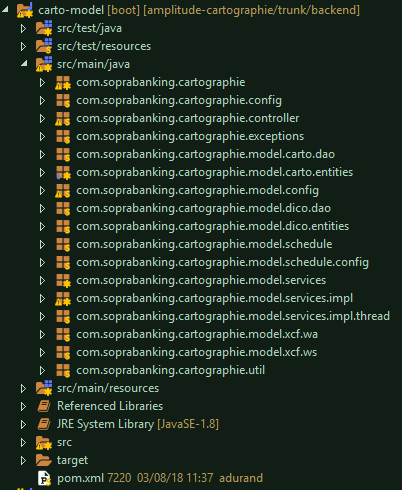
\includegraphics[scale=1]{images/arboBackEnd}
	\caption{Arborescence du \textit{back-end} de l'outil de cartographie}
	\label{fig:arboBackEnd}
\end{figure}

La structure de la partie \textit{back-end} reprend une arborescence classique de projet Java, avec les sources séparées en deux packages principaux: \textbf{main} pour les fichiers de sources et \textbf{test} pour les fichiers de tests unitaires. On peut voir la présence du fichier \textit{pom.xml} à la racine du projet et qui contient les dépendances nécessaires pour notre outil. Parmi les dépendances (voir la \autoref{sec:utilisationMaven} pour comprendre le fonctionnement), on retrouve les starters de \textit{Spring Boot} (\textit{spring-boot-starter-data-jpa}, \textit{spring-boot-starter-web}, \textit{spring-boot-starter-test}), deux dépendances pour \textit{Spring Security}, les drivers pour les connexions à la base de données (une pour notre base sous \textit{Oracle} et une pour la base du dictionnaire de données sous \textit{Informix}).

Ensuite, dans les sources présentes dans le package \textbf{main}, les fichiers Java sont répertoriés dans un package principal \textit{com.soprabanking.cartographie}. À la racine, nous avons le fichier \textbf{main} du programme et les packages suivants : 

\begin{description}
	\item[controller] qui contient deux classes de contrôleur, une pour la partie Dictionnaire et une pour la partie Cartographie. Ce sont ces deux contrôleurs qui vont exposer les données en REST au \textit{front-end}. 
	\item[exceptions] avec les exceptions pour certains cas de figure.
	\item[model] avec toute la gestion des données de l'outil: les classes d'entités de \textit{Spring Data}, les \textit{repositories}, la gestion du job d'alimentation et les services \textit{Spring Data}.
	\item[util] qui contient les classes utilitaires comme par exemple, la gestion des connexions SVN.
\end{description}

Comme expliqué, on retrouve de nombreux éléments différents dans la partie \textbf{model} qui respectent la structure suivante : 

\begin{description}
	\item[carto] contient les entités de la cartographie technique (programmes, modules 4GL, fonctions techniques, ...) et leurs \textit{repositories} respectifs permettant la gestion des données avec \textit{Spring Data}
	\item[dico] contient les entités du dictionnaire des données (domaines, fonctions, sous-fonctions, tables, ...) et leurs \textit{repositories} respectifs permettant la gestion des données avec \textit{Spring Data}
	\item[config] contient deux classes de configuration pour les transactions vers les bases de données.
	\item[schedule] contient les éléments du job d'alimentation.
	\item[xcf] contient les classes pour l'extraction du dictionnaire des programmes.
\end{description}

Les fichiers de ressources contenant les propriétés de l'application et du job d'alimentation sont contenus dans le package \textbf{main/resources}.

Du côté \textit{Angular}, la structure reprend celle d'un projet \textit{Angular} classique dont nous verrons plus de détails dans le \autoref{chap:frontEnd}.

L'empaquetage de l'application se fait par \textit{Maven}. Nous avons donc un projet parent et deux projets fils, le tout relié par \textit{Maven}. Le côté \textit{back-end} se comporte comme un projet \textit{Maven} classique, tandis que le côté \textit{front-end}, lors de son déploiement, installe au préalable les dépendances et les outils nécessaires au fonctionnement d'\textit{Angular} (\textit{Angular-cli}, \textit{npm}, \textit{ng}, tous les éléments détaillés dans le \autoref{chap:angular}). Ainsi, au déploiement de l'application, les deux sous-projets sont déployés chacun de leur côté. 

\chapter{Exposition REST des données}

\section{Principe du REST}

L'un des points central de notre outil est l'exposition des données de la partie \textit{back-end} à la partie \textit{front-end}. Et l'exposition des données se fera par le biais d'une architecture REST. Le REST (Representational State Transfer) est un style d'architecture permettant de construire des applications. Il s'agit davantage d'un ensemble de conventions et de bonnes pratiques plutôt qu'une technologie à part entière. Cette architecture utilise les spécifications originelles du protocole HTTP. 

REST se base sur les URI (Uniform Resource Identifier) afin d’identifier une ressource. Ainsi une application se doit de construire ses URI (et donc ses URL) de manière précise, en tenant compte des contraintes REST. Il est nécessaire de prendre en compte la hiérarchie des ressources et la sémantique des URL pour les éditer. Dans notre cas par exemple, pour récupérer l'ensemble des domaines présents dans le dictionnaire des données, nous pouvons utiliser l'URL : \javacode{/dico/domaines}. Pour en récupérer un avec un identifiant précis, on utilise l'URL : \javacode{/dico/domaines/\{id\}} avec l'identifiant que l'on souhaite.

Ensuite, la gestion des ressources se fait en utilisant des requêtes HTTP. Ainsi, on peut effectuer 4 opérations (les 4 opérations du CRUD) :

\begin{itemize}
	\item Créer (create) $\Rightarrow$ \textbf{POST}
	\item Afficher (read) $\Rightarrow$ \textbf{GET}
	\item Mettre à jour (update) $\Rightarrow$ \textbf{PUT}
	\item Supprimer (delete) $\Rightarrow$ \textbf{DELETE}
\end{itemize}

Une exemple avec notre outil, une mise à jour d'un programme de la cartographie se fera avec une requête \textbf{PUT} sur l'URL \javacode{/carto/programmes/\{id\}} avec l'identifiant du programme que l'on souhaitera modifier.

\section{Implémentation avec \textit{Spring Data}}

L'implémentation du REST avec \textit{Spring Data} se fait facilement à l'aide des différentes annotations à disposition. Tout d'abord, il faut préciser que les contrôleurs de l'application prennent en compte le REST avec l'annotation \javacode{@RestController}. Ensuite, il faut indiquer \textit{Spring} le \textit{mapping} de l'application, en d'autres termes, les URL qui seront utilisées pour le partage des ressources. Le \textit{mapping} se fait avec des annotations \javacode{@RequestMapping} sur la classe du contrôleur pour indiquer le contexte général, puis sur les méthodes qui vont gérer les ressources. La \autoref{fig:restController} montre une implémentation de l'architecture REST.

\begin{figure}
	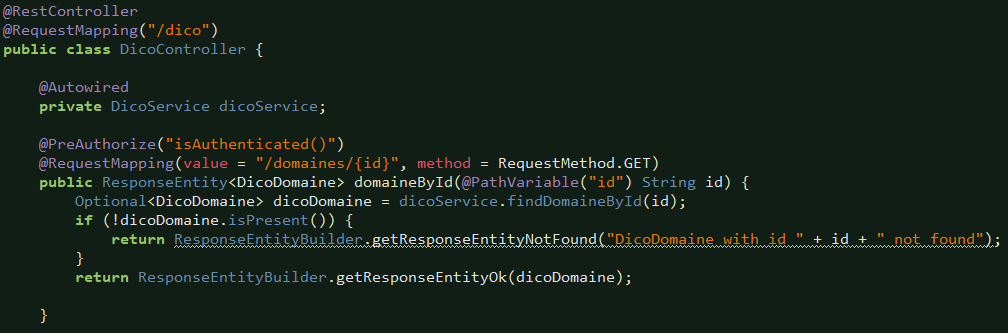
\includegraphics[scale=0.65]{images/restController}
	\caption{Prise en charge du REST avec \textit{Spring Data}}
	\label{fig:restController}
\end{figure}

On peut voir sur l'illustration l'annotation \javacode{@RequestMapping("/dico")} qui précède la déclaration du contrôleur ainsi que l'annotation \javacode{@RequestMapping("/domaines/\{id\}")} avant la déclaration de la méthode qui récupère un domaine selon l'identifiant. Ainsi, il est possible de retrouver les domaines que l'on souhaite par le biais de l'URL : \javacode{/dico/domaines/\{id\}}. 

\chapter{Gestion du job d'alimentation}


L'un des aspects principales de l'outil est l'alimentation des différents ressources. Le processus d'alimentation doit nous permettre de récupérer les éléments de la cartographie technique, les données du dictionnaires des données nous sont déjà directement accessibles depuis la base de données. L'alimentation et la mise à jour des ressources doit se faire régulièrement, pour avoir la meilleure cartographie possible à un instant T. Nous avons choisi de l'effectuer tous les jours à minuit, pour permettre d'avoir la bonne cartographie chaque jour. 

Pour la gestion du processus d'alimentation, nous avons utilisé la bibliothèque open-source \textit{Quartz}. Elle permet de programmer des processus pour qu'ils se lancent au moment que l'on souhaite. La mise en place d'un job se fait avec à minima deux fichiers : un décrivant le job et l'autre contenant les configurations. Le fichier qui décrit le processus à accomplir doit implémenter l'interface \textit{Job} de la bibliothèque \textit{Quartz}. Ensuite la classe doit avoir une méthode \javacode{execute()} qui indique les traitements à effectuer. La configuration du job se trouve dans une classe qui précise les détails du job et qui met en place le déclencheur du processus (le \textit{trigger}). 

Pour notre outil de cartographie, le job va appeler les méthodes de récupération d'\textit{Amplitude} avec SVN et d'alimentation des données par la suite. La \autoref{fig:serviceJob} représente l'implémentation dans la classe \textit{AlimentationCartoService} de l'appel aux méthodes d'alimentation.


\begin{figure}
	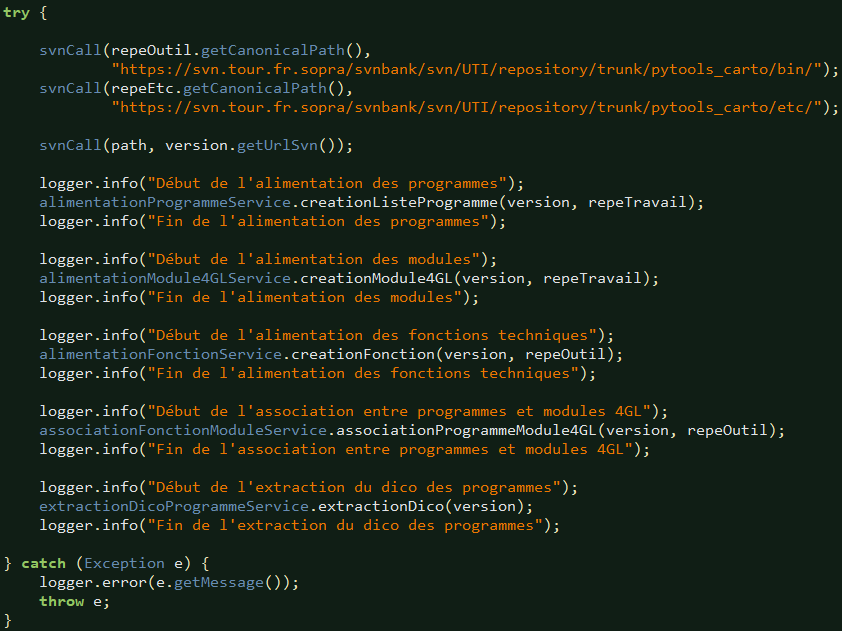
\includegraphics[scale=0.7]{images/serviceJob}
	\caption{Implémentation des méthodes d'alimentation}
	\label{fig:serviceJob}
\end{figure}

Comme on le voit sur l'image, les méthodes appelées sont les suivantes :

\begin{itemize}
	\item Des appels à la méthode \textit{svnCall()} pour récupérer les outils de développement d'\textit{Amplitude} (pour utiliser le script python pour la récupération des fonctions techniques notamment;
	\item Un appel à la méthode \textit{svnCall()} pour récupérer les sources \textit{Amplitude} pour la version indiquée en paramètre;
	\item Un appel à la fonction de création des programmes;
	\item Un appel à la fonction de création des modules 4GL;
	\item Un appel à la fonction de créations des fonctions techniques;
	\item Un appel à la fonction d'associations des programmes et des modules 4GL;
	\item Un appel à la fonction d'extraction du dictionnaire des programmes;
	\item Un appel à la fonction de récupération des SMG.
\end{itemize}

La fonction \javacode{svnCall()} effectue un \textit{checkout} des sources dans le cas où il s'agit de la première alimentation ou un \textit{update} dans le cas où les sources sont déjà présentes. 

Les méthodes sont appelées une à une de façon séquentielle. La question du multi-threading s'est posée pour améliorer les temps de traitements. En effet, la création initiale des entités en base peut prendre beaucoup de temps. La création des programmes et des modules se fait relativement rapidement tandis que la création des fonctions prend à l'heure actuelle, un temps qui n'est pas concevable pour une mise en production (aux alentours de 10 heures de traitement). Cela est dû à l'utilisation du script Python \textit{check\_func\_xl.py} qui nécessiterait une amélioration et au fait que chaque programme lance une instance de Python avec une exécution de script. Ainsi, nous avons mis en place un multi-thread sur ces traitements, ce qui permet de prendre en charge plusieurs scripts en simultané. 


\chapter{Gestion du front-end et de la sécurité}
\label{chap:frontEnd}

La partie \textit{front-end} et la gestion de la sécurité a été pris en charge par les architectes. Je ne vais donc pas rentrer dans les détails des implémentations mais plutôt évoquer le fonctionnement général de ces aspects.

\section{Gestion de la sécurité}

L'outil final pourrait être accessible à de nombreuses personnes au sein de l'entreprise une fois la mise en production. La nécessité de sécuriser la plate-forme est présente étant donné qu'il est possible de manipuler des données faisant parties intégrantes de la cartographie. Une modification même minime sur les données pourrait entraîner des problèmes, notamment si cela touche des données associées avec plusieurs entités.

Les authentifications à la plateforme sont gérées avec le framework \textit{oauth2}. C'est un framework qui permet de limiter les accès d'un compte sur les services HTTP. Il est utilisé par de nombreux sites réputés comme \textit{Facebook} ou \textit{Github}. L'utilisation du framework sur notre application est gérée automatiquement par \textit{Spring Security}. La gestion des authentifications à l'aide de jetons attribués à un compte une fois celui-ci connecté. 

On peut voir sur la \autoref{fig:restController} dans le chapitre précédent la présence de l'annotation \javacode{@PreAuthorize("isAuthentificated()")}. Celle-ci permet de refuser l'accès à la méthode si le visiteur ne s'est pas authentifié au préalable. 

\section{Aperçu de l'affichage}

Les deux images suivantes montrent un aperçu du rendu de l'outil de cartographie. La première page que l'on trouve lorsque l'on souhaite utiliser l'outil est la \autoref{fig:cartoLogin}, la page d'authentification. Une fois authentifié, nous arrivons sur la page d'accueil de l'application que l'on peut voir sur la \autoref{fig:cartoAccueil}. L'aperçu de la page d'accueil ici est provisoire, néanmoins la structure finale sera la même, à savoir un aperçu des domaines de la cartographie fonctionnelle. Un clic sur une tuile représentant un domaine permet d'avoir un visuel du contenu de l'entité. 

\begin{figure}
	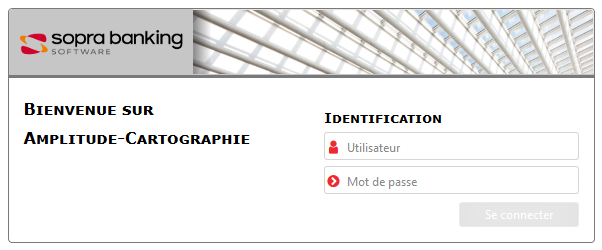
\includegraphics[scale=0.8]{images/cartoLogin}
	\caption{Page d'authentification de l'outil de cartographie}
	\label{fig:cartoLogin}
\end{figure}


\begin{figure}
	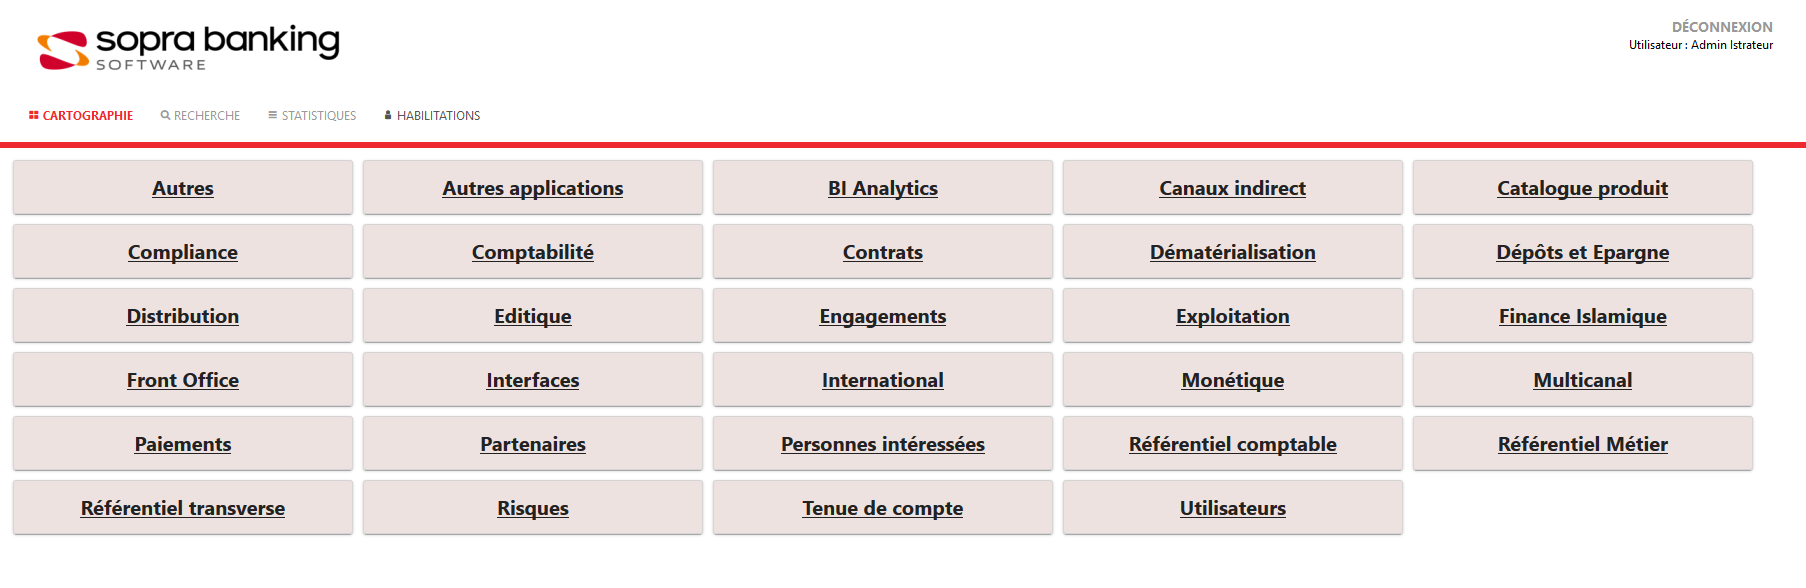
\includegraphics[scale=0.33]{images/cartoAccueil}
	\caption{Page d'accueil de l'outil de cartographie}
	\label{fig:cartoAccueil}
\end{figure}

Parmi les autres éléments notables de la page d'accueil, on peut retrouver les onglets \textit{Recherche}, \textit{Statistiques} et \textit{Habilitations}. L'onglet de recherche, comme son nom l'indique, permet de rechercher un élément que l'on souhaite analyser. L'onglet \textit{Statistiques} va regrouper différentes informations générales comme les fonctions inutilisées, les modules les plus utilisés, etc.. Les habilitations seront accessibles uniquement pour les administrateurs de l'outil. 

Ces éléments ne sont pas encore intégrés et seront les prochaines étapes de développement dans le futur. 

\chapter*{Bilan du stage}


À l'heure où s'achève mon stage, le moment est venu de dresser le bilan de ces derniers mois. Dans un premier temps, concernant l'état du projet à l'issue du stage, nous avons respecté les délais fixés par les chiffrages de développement. Après l'analyse de l'expression des besoins, nous savions que les temps pour finir intégralement seraient très courts et qu'il serait quasiment impossible de terminer l'outil à la fin du mois d'août. Néanmoins, notre objectif était d'avoir au moins la partie \textit{back-end} de l'application fonctionnelle, ce qui est le cas. Des améliorations sont cependant encore nécessaires, notamment en ce qui concerne les temps de traitement pour l'alimentation des données.

D'un point de vue personnel, ce stage a été pour moi l'expérience professionnelle la plus enrichissante que j'ai connu, et de loin, et cela pour plusieurs raisons. Tout d'abord, ça a été la première fois pour moi d'être intégré dans un projet à plein temps sur une période aussi longue. Ensuite, le sujet était particulièrement complet et m'a permis de voir de toucher à de nombreux aspects de la vie d'un ingénieur. Commencer par comprendre les besoins du "client" pour ensuite modéliser une solution qui convient avant de la mettre en œuvre était vraiment intéressant. La variété aussi bien des tâches à accomplir que des technologies utilisées a fait que je n'ai jamais ressenti de moments d'ennui ou de lassitude pendant le stage, ce qui peut parfois arriver pour certains étudiants-ingénieurs.

Pour conclure, je tiens à remercier mon encadrant, M. Alexandre DURAND, qui m'a fait confiance dès le passage des portes de \textit{Sopra Banking Sotware} lors de mon premier entretien jusqu'à mes derniers jours de stage et même dans un futur proche en me proposant un contrat de travail. J'espère pouvoir ainsi terminer cet outil de cartographie et qu'il soit utile au plus grand nombre dans l'entreprise. Je voudrais ensuite remercier mes collègues pour l'intégration dans la cellule dès les premiers jours, pour la bonne ambiance qui règne au quotidien et pour leur humour à toute épreuve ! Et enfin merci à Polytech pour ses années d'étude qui vont me permettre de rentrer dans la vie active de la meilleure des façons.

\appendix

\chapter{Diagramme de classe}
\label{ann:diagClasse}

\begin{landscape}
	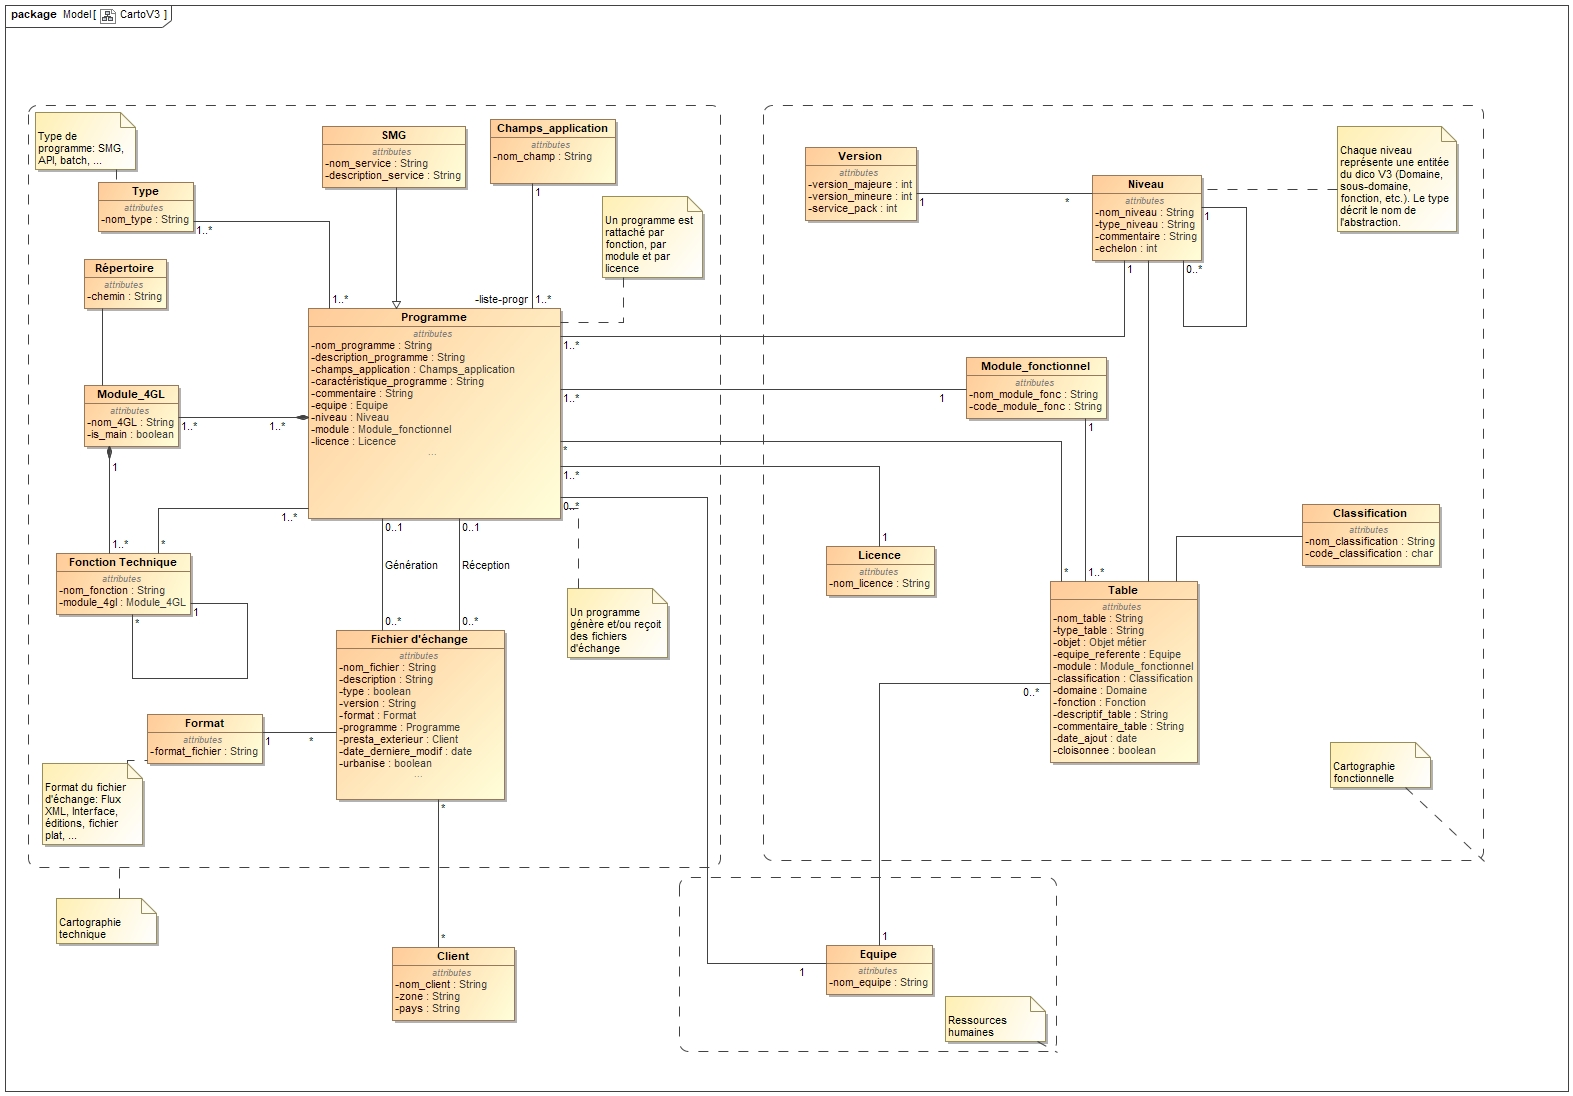
\includegraphics[scale=0.37]{images/CartoV3}
\end{landscape}

\end{document}
